\documentclass[dvipdfmx,8pt]{beamer}
\usepackage{bxdpx-beamer} % dvipdfmxなので必要
\usepackage{pxjahyper} % 日本語のしおり用
% \usepackage{minijs} % フォントの設定?pLaTeX, upLaTaXなら不要

\usepackage{url} % 文中にリンク張る用
\usepackage{amsmath} %数式用
\renewcommand{\kanjifamilydefault}{\gtdefault} % 既定をゴシック体に変更


% \usetheme{metropolis}
\AtBeginSection{\frame{\sectionpage}} % Section毎に見出しを追加

\title{The Elements of Statistical Learning\\Chap.14: Unsupervised Learning}
\date{\today}
\author{Kosuke Kito}

\begin{document}
  \maketitle
  \begin{frame}{流れ}
    \begin{itemize}
      \item 導入
      \item アソシエーション分析
      \item クラスター分析
      \item 自己組織化マップ
      \item 主成分, 主曲線, 主面
      \item 非負行列分解
      \item 独立成分分析と探索的射影追跡
      \item 多次元尺度構成法
      \item 非線形次元削減と局所多次元尺度構成法
    \end{itemize}
  \end{frame}
  \section{導入\\p.485-}
  \begin{frame}{導入}
    \begin{itemize}
      \item 教師あり学習
        \begin{itemize}
          \item 変数$X$, $Y$に関する訓練データ$\{(x_1,y_1), \dots , (x_N, y_N)\}$から,
          条件付確率分布$\mathrm{Pr}(Y|X)$を推定する.

          \item 特に, 損失を最小化する条件付き期待値
          \[
            \mu(x)=\mathrm{arg}\min_{\theta} \mathrm{E}_{Y|X}L(Y,\theta)
          \]
          に興味がある.

          \item 推定の成功度合いを測りやすい

        \end{itemize}

      \item 教師なし学習
        \begin{itemize}
          \item 変数$X$に関する訓練データ$\{x_1 , \dots , x_N\}$から,
          確率分布$\mathrm{Pr}(X)$を推定する.

          \item 一般に, 変数$X$の次元は教師ありと比べて非常に大きい.

          \item 興味の対象は期待値に限らず, 様々. 複雑.

          \item 成功度合いを測りにくい→多数の手法が提案されている.
          乱立状態?(heavy proliferation)
        \end{itemize}
    \end{itemize}
  \end{frame}
  \section{アソシエーション分析\\p.487-}
  \begin{frame}{アソシエーション分析}
    出現頻度の高い変数の値の組み合わせを発見するための手法.
    イメージは, スーパーでよく一緒に買われる商品探し.
    \begin{itemize}
      \item 基本形は, 以下の通り. (mode finding, bump hunting)

      変数$X=(X_1,\dots,X_p)$に対して, $X$のとりうる値$v_l$で, 確率$\mathrm{Pr}(X=v_l)$が
      比較的大きいものの集まり$v_1,\dots,v_L$を見つける.
      \item 各$i$について, $X_i\in\{0,1\}$というデータに適用することが多い.
      \item 二値データでない場合も, ダミー変数を使って, 二値データに変形できる.
      (次元はめっちゃ大きくなる. )
      この変形をしたデータは$Z$と書く.
      \item 推定は, 実際に訓練データのうち, その値を取るものの数を数えればいいので, 簡単.
      \item 変数の次元が高く, 定義域が広いときには, 信頼できる推定ができなくなる.

      →一点の確率ではなく, 領域の確率を考えるとよい. (全ての変数の値を指定しない, ということ. )
    \end{itemize}
  \end{frame}
  \begin{frame}{アソシエーション分析 - 領域版}
    ``一点の確率ではなく, 領域の確率を考える''とは, 以下の通り.

    各$X_i$に対して, その値域の部分集合$s_i$(support)を
    とった組$s_1,\dots,s_p$で,
    \[
      \mathrm{Pr} \left (\bigcap_{j=1}^p\{X_j \in s_j\} \right )
    \]
    が比較的大きいものを探す.
  \end{frame}
  \begin{frame}{アソシエーション分析 - Aprioriアルゴリズム}
    領域版かつ二値データのアソシエーション分析で, 領域を発見するためのアルゴリズム.

    準備

    変数が$K$個とする.
    $\mathcal{K}\subset\{1,\dots,K\}$に対して,
    \[
      T(\mathcal{K})=\hat{\mathrm{Pr}}\left( \prod_{k\in\mathcal{K}}\{Z_k=1\}  \right)=\frac{1}{N}\sum_{i=1}^N\prod_{k\in\mathcal{K}}z_{ik}
    \]
    とする. これは, データが領域$\mathcal{K}$に入る確率の推定値.
    これが大きい領域を見つけたい.

    \begin{enumerate}
      \item 閾値$t$を決める.
      \item $L_1=\{|\mathcal{K}|=1, T(\mathcal{K})>t\}$
      \item $i>=2$について, $L_i$が空になるまで4を繰り返す.
      \item $L_i=\{|\mathcal{K}|=i, T(\mathcal{K})>t, \mathcal{K}\setminus\{k\}\in L_{i-1} \forall k \in \mathcal{K}\}$
      \item $L_i$たちの和集合を出力する.
    \end{enumerate}
  \end{frame}
  \begin{frame}{アソシエーション分析 - 3つの指標}
    Aprioriアルゴリズムで, 良い領域が見つかった後の処理について.
    3つの指標を考える.
    $\mathcal{K}$をAprioriアルゴリズムで出てきた領域の一つとする.
    これを, 2つに分割する.
    \[
      A \cup B = \mathcal{K}, A \cap B = \emptyset
    \]
    で, association ruleを,
    \[
      A \Rightarrow B
    \]
    と書く. これは, Aだったときに, Bである, くらいの意味.

    以下指標.
    \begin{itemize}
      \item 支持度(support)
        \[
          T(A \Rightarrow B)=T(A \cup B)
        \]
      \item 確信度(confidence)
        \[
          C(A \Rightarrow B)=\frac{T(A \Rightarrow B)}{T(A)}
        \]
        これは, ほぼほぼ条件付き確率$\mathrm{Pr}(B|A)$.
      \item リフト値(lift)
        \[
          L(A \Rightarrow B)=\frac{C(A \Rightarrow B)}{T(B)}
        \]
        Aの中のBの割合と, 全体の中のBの割合の比率.
    \end{itemize}
    この3つを見て, 因果関係を推測するのが, アソシエーション分析のゴール.
    特に, 支持度と確信度の高いassociation ruleを見つけたい.

  \end{frame}
  \begin{frame}{アソシエーション分析 - Aprioriアルゴリズムの後}
    Aprioriアルゴリズムの結果出てきた各集合$\mathcal{K}$と$A\subset
    \mathcal{K}$について, 確信度を計算すれば, 良い.

    ただし, これについては, 効率的な方法が提案されているとか.

    ``Associaton rules are among data mining's biggest success''らしいので,
    すごいっぽい.

  \end{frame}
  \begin{frame}{アソシエーション分析 - 問題点}
    \begin{itemize}
      \item 最初にAprioriアルゴズムで, 一定以上の出現頻度の組み合わせに絞っている.
      \item 閾値を下げると, 計算量は指数的に増大する.
    \end{itemize}
    →めったに起きないが, 起きるときには決まって一緒に起きるような事象の組を発見できない.
  \end{frame}
  \section{クラスター分析\\p.501-}
  \begin{frame}
    訓練データを, グルーピングする手法.
    同一グループ内の``類似度''を高くして, 異なるグループ間での``類似度''を低くしたい.

    そのためには, ``類似度''を定める必要があり, これがクラスター分析の肝でもある.
  \end{frame}
  \begin{frame}{クラスター分析 - (非)類似度}
    $N$件のデータに対して, $N \times N$行列$\textbf{D}$で, $\textbf{D}_{ij}$が
    訓練データ$x_i$と$x_j$の(非)類似度になっている行列を入力とする分析手法が多いらしい.
    (この行列は対称行列になる. )

    で, $X_i$と$X_j$の非類似度として, 各次元の非類似度の和を使ったりする.
    \[
      \textbf{D}_{ij}=\sum_{k=1}^pd_k(x_ik, x_jk)
    \]
    例えば, 差の二乗和でユークリッド距離とか.

    詳しく見ていく. まず, 各次元(attribute)の非類似度はどう決まるのか.

    \begin{itemize}
      \item 量的変数の場合

      一般的には, 差の絶対値を, 単調増加関数に食わせたものを使えばよい.
      \[
        d(x_i, x_{i'})=l(|x_i-x_{i'})
      \]
      差の二乗は典型例.

      そもそも, $p$個の変数の相関係数を類似度として採用してしまうのもあり.
      \item 順序付き質的変数の場合

      連続した整数とかで表すことが多い.

      \item 質的変数の場合

      一緒なら0, 違うなら1にしてしまうのことが多い.
      特に大きな違いがあるものの差を大きくしたりすることもあるとか.

    \end{itemize}
  \end{frame}
  \begin{frame}{クラスター分析 - (非)類似度}
    次に, 全体の非類似度の決め方

    上記の通り, 単純な和もあり. 重み付けても良し. (subject matter consideration)

    ただし, 全次元を同程度重視する重みは, 定数ではない.
    \[
      w_j\sim \frac{1}{\sum_i\sum_{i'}d_j(x_{ij},x_{i'j})}
    \]

    この重みの掛け方がいい感じだが, 逆効果になるケースもある.
    実際問題, 特定の変数の際がクラスタリングにとってとても重要なケースもあるよね, ということらしい.

    結局, 適切な類似度の数値化は, ケースバイケースで
    判断するしかないみたい.
    \begin{figure}[htb]
      \centering
      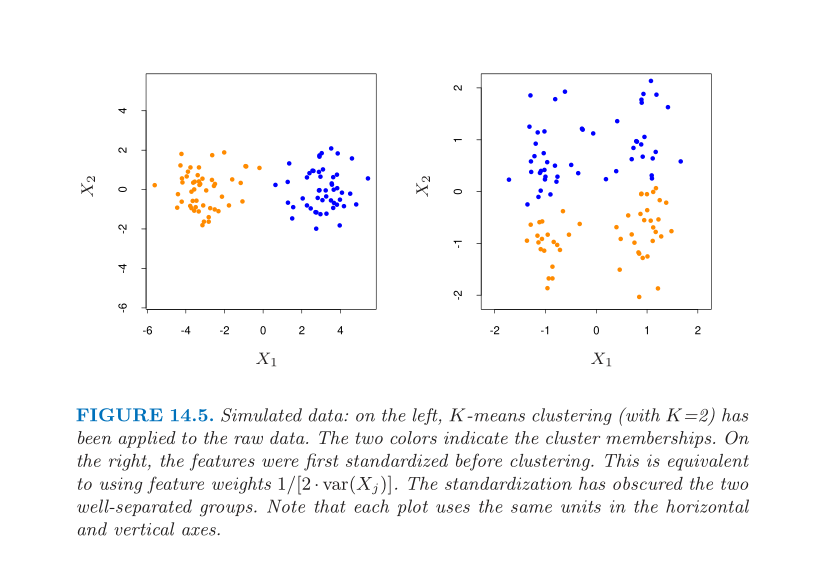
\includegraphics[width=5cm,clip]{images/missclustering.png}
    \end{figure}
  \end{frame}
  \begin{frame}{クラスター分析 - 欠損値}
    類似度行列を作る際に, 欠損値にどう対応するか.
    \begin{itemize}
      \item 欠損のある項目は無視. 共通して持っている項目がないなら, データごと無視.
      \item 欠損している箇所は平均値, 中央値で代替.
      \item 質的変数については, 欠損という新しい値として扱ってもよい. (欠損が一つの特性と考えられる場合のみ)
    \end{itemize}
  \end{frame}
  \begin{frame}{クラスター分析 - アルゴリズム}
    代表的なアルゴリズムが3種類.
    \begin{itemize}
      \item combinatorial algorithm

        確率分布とかを考えずに, データを見ていく
      \item mixture modeling

        確率分布を考えてデータを見ていく
      \item mode seeker

        分布の最頻値(極大値?)を探す
    \end{itemize}

  \end{frame}
  \begin{frame}{クラスター分析 - combinatorial algorithm}
    $N$このデータを$K<N$このクラスターに分けるのは, 関数
    \[
      C \colon \{1,\dots,N\} \to \{1,\dots,K\}
    \]
    とみなせる. このような関数でいい感じのものを見つけるのが, 今回の手法.

    ``いい感じ''とは, 同一クラスター内の類似度が高いもの.
    前出のの非類似度を使うと, 以下の最小化を考えるということ.
    \[
      W(C)=\frac{1}{2}\sum_{k=1}^K\sum_{C(i)=k}\sum_{C(i')=k}d(x_i,x_{i'})
    \]

    全体の非類似度の総和
    \[
      T=\frac{1}{2}\sum_{i=1}^N\sum_{i'=1}^Nd_{ii'}
    \]
    は定数なので, 以下の最大化と等価.
    \[
      B(C)=\frac{1}{2}\sum_{k=1}^K\sum_{C(i)=k}\sum_{C(i')\ne k}d(x_i,x_{i'})
    \]

    Wは``within cluster point scatter''\\
    Bは``between cluster point scatter''\\
    の頭文字.
  \end{frame}
  \begin{frame}{クラスター分析 - K平均法}
    さっきの最小化は, 候補が多すぎて総当たりは厳しい. \\
    →いい感じの反復的なアルゴリズムが欲しい. \\
    →K平均法の出番.

    前提条件
    \begin{itemize}
      \item 入力変数はすべて量的である.
      \item 非類似度は(重み付き)ユークリッド距離である.
    \end{itemize}
    このとき, $W(C)$は,
    \[
      W(C)=\frac{1}{2}\sum_{k=1}^K\sum_{C(i)=k}\sum_{C(i')=k}d(x_i,x_{i'})=\sum_{k=1}^KN_k\sum_{C(i)=k}|x_i-\bar{x}_k|^2
    \]
    と書ける. ただし, $\bar{x}_k$は, クラスター$k$に分類されたデータの平均値. $N\_k$は個数.

    これを最小化する, ということは平均からの距離でクラスターを決定するといいうことなので,
    平均を取る→分ける→平均を取る→分ける→$\cdots$という反復アルゴリズムが正当化される.
  \end{frame}
  \begin{frame}{K平均法}
    \begin{figure}[htb]
      \centering
      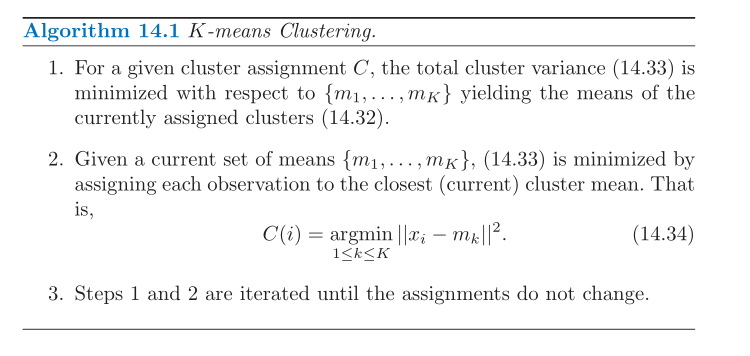
\includegraphics[width=10cm,clip]{images/kmeans.png}
    \end{figure}

    ちなみに, K-meansの結果はVoronoi tessellationというものになる.
    k-NNの$k=1$の時と似てるけど, 混同しないように.

    それと, 平均を取る→分けるの繰り返しは, EMアルゴリズム(expectation–maximization)とそっくり.
    実際, EMアルゴリズムはK平均法を和らげたものと思えるらしい.
  \end{frame}
  \begin{frame}{クラスター分析 - ベクトル量子化}
    複数のアナログデータをまとめてデジタルデータ化(量子化)したいとき, K平均法が活躍するらしい.
  \end{frame}
  \begin{frame}{クラスター分析 - K-medoids}
    K平均法を, ユークリッド距離以外や質的データにも使うために, 一般化した方法.

    各クラスタの代表点として, 平均ではなく他との非類似度との和が最小の点を取る.
    \begin{figure}[htb]
      \centering
      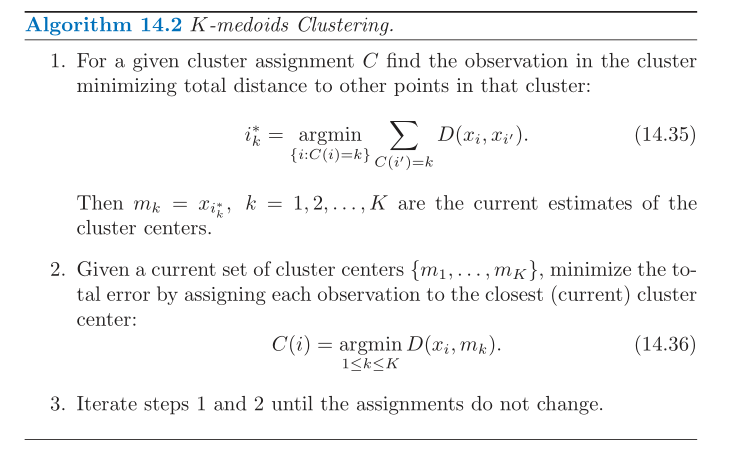
\includegraphics[width=10cm,clip]{images/kmedoids.png}
    \end{figure}
  \end{frame}
  \begin{frame}{クラスター分析 - Practical Issues}
    K平均法やK-medoidsを使う場合, $K$の値と, 各クラスターの代表値の初期値を決めてあげないといけない.
    \begin{itemize}
      \item 各クラスターの代表値の初期値について

      これは, まぁ, 一個ずつ順に遠くになるようにとってあげればよい.

      \item $K$の値について
      \begin{itemize}
        \item この値は, データからではなく, 分析の目的によることも多い.
        \item 一方, $K$自体も推定の対象であることもある. 以下$K$の推定について.

        \item クラスターを増やすほど, テストデータへの適合度も上がるので, 交差検証は使えない.

        \item $K$が小さすぎるときは, $K$を1増やすと, 効果が大きそう.
        一方, $K$が十分大きければ, $K$を増やしても大した効果はなさそう. \\
        →$K$を変化させて, $W$の変化を見ればよいかも.
      \end{itemize}
    \end{itemize}
  \end{frame}
  \begin{frame}{クラスター分析 - 階層的クラスタリング}
    K平均法とは全然違うクラスタリングの考え方.
    前提として, 任意の共通部分のないデータの集合間の非類似度を測れる必要がある.

    結果を図示した以下のような図ををデンドログラムという.
    \begin{figure}[htb]
      \centering
      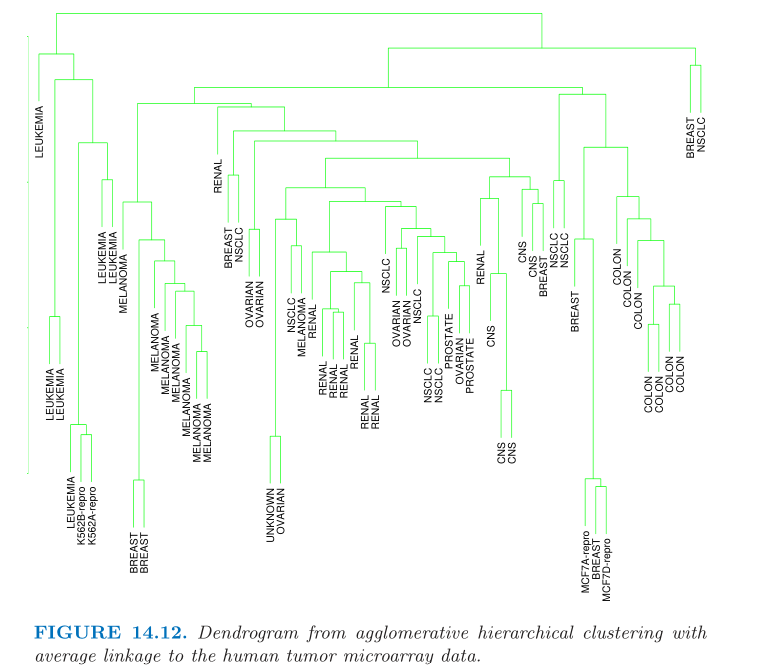
\includegraphics[width=8cm,clip]{images/dendrogram.png}
    \end{figure}
  \end{frame}
  \begin{frame}{クラスター分析 - 階層的クラスタリングのアルゴリズム}
    大きく分けて2つの考え方がある.
    \begin{itemize}
      \item agglomerative(bottom up)

      デンドログラムをしたから作っていくイメージ.
      一番近いものを順に括っていく.
      \item divisive(top down)
      デンドログラムを上から作っていくイメージ.
      一番離れるように分けていく.
    \end{itemize}

    階層的クラスタリングの評価は, ``cophenetic相関係数''というものが使われる.
    これは, 各データの組$x_i$,$x_j$に対する, 非類似度$d_{ij}$とデンドログラム上で
    これらが合流する時の非類似度$C_{ij}$の相関係数.
  \end{frame}
  \begin{frame}{クラスター分析 - agglomerative clustering}
    階層的クラスタリングの具体的方法1, bottom upの方法.
    方法は至極単純.

    \begin{enumerate}
      \item まず, 各データをそれのみからなるクラスターとして, $K=N$の状態から始める.
      \item 既存のクラスターのうち, 最も近い2つをまとめる. クラスター数が1個減る.
      \item 2をN-1回繰り返す.
    \end{enumerate}

    問題は, クラスターの近さをどう測るか. 方法がいくつか. $G$, $H$をクラスターとする.
    \begin{itemize}
      \item single linkage(SL): 緩い
        \[
          d_{\mathrm{SL}}(G,H)=\min_{i\in G, i'\in H}d_{ii'}
        \]
      \item complete linkage(CL): 厳しい
        \[
          d_{\mathrm{CL}}(G,H)=\max_{i\in G, i'\in H}d_{ii'}
        \]
      \item group average(GA): 中間, 単調変換に弱い
        \[
          d_{\mathrm{GA}}(G,H)=\frac{1}{N_GN_H}\sum_{i \in G, i'\in H}d_{ii'}
        \]
    \end{itemize}
  \end{frame}
  \begin{frame}{クラスター分析 - divisive clustering}
    階層的クラスタリングの具体的方法2, top downの方法.
    あまり研究されていないらしい.

    方法としては, K平均法やK-medoidsを$K=2$として繰り返し適用する感じ. \\
    →別れ方が各繰り返しの初期値による.
    また, クラスター間の距離が単調にならず, デンドログラムが書けない可能性あり. \\
    →この問題を避ける方法が提案されている.

    各繰り返しで, 以下の方法によりクラスター$G$を$G$, $H$に分割する.
    \begin{enumerate}
      \item $G$の中で, 他のデータとの非類似度の平均が最大のものを$H$に移す.
      \item $G$の中で, $(H\mbox{内のデータとの非類似度の平均})-(G\mbox{内の他のデータとの非類似度の平均})$が最大のものを$H$に移す.
      \item 2を非類似度の平均の差が府になるまで繰り返す.
    \end{enumerate}

    問題は, 各繰り返しで, 既存のクラスターのどれを分割するか. 方法が二つ.
    \begin{itemize}
      \item 直径が最大のクラスターを分割する.
      \item クラスタ内の平均非類似度が最大のクラスターを分割する.
    \end{itemize}
  \end{frame}
  \section{自己組織化マップ\\p.528-}
  \begin{frame}{自己組織化マップ}
    K平均法に, 各クラスターの代表点たちが1, 2次元の空間上にいる, という制限を加えたもの, と思える方法.

    操作のイメージわきにくいと思う. 下のサイト, イメージ持つにはよさそうでした.
    \url{http://gaya.jp/spiking_neuron/som.htm}

    Manifold: 多様体. 局所的にはユークリッド空間と思える空間. 球面とか, ドーナツとか.
  \end{frame}
  \begin{frame}{自己組織化マップ}
    さっきの例は色を変えていったが, 今回の例は, 代表点の座標を変えていく.

    \begin{itemize}
      \item 格子点$l_j\in\{1,\dots,q_1\}\times\{1,\dots,q_2\}$と,
        それに対応する変数空間の格子点$m_j$を取る.
        $m_j$たちは, 例えば, 2次元の主成分平面(後述)に取ればよい.
      \item 以下をいい感じに繰り返す.
      \begin{itemize}
        \item 各$x_i$について, $x_i$に一番近い$m_j$とその近傍の$m$たち全員を$x_i$の方に動かす.
          \[
            m_k = m_k + \alpha(x_i-m_k)
          \]
          ただし, 近傍とは, 対応する$l$の距離が閾値$r$以下のもの.
      \end{itemize}
    \end{itemize}
    これがなぜだかうまくいくのは, さっきの動画の通り.

    $\alpha$と$r$の決め方について.

    $\alpha$は$1$から$0$に徐々に減少させていき,
    $r$は適当な$R$から$1$へ減少させていくやり方は良くある.

    点の移動の強化について.
    \[
      m_k = m_k + \alpha h(|l_j-l_k|)(x_i-m_k)
    \]

    $r$が小さすぎるとき, K平均法と等価になるらしい.
  \end{frame}
  \section{主成分, 主曲線, 主面\\p.534-}
  \begin{frame}{次元削減}
    \begin{columns}[t]
      \begin{column}{0.5\textwidth}
        \begin{itemize}
          \item 本節での学習の目的は, ``次元削減''(dimention reduction).
          \item 発想は, ``たくさんのデータ取っているけど, 実際はより少数のパラメータで大部分を説明できるよね''というもの.
          \item 専門用語を使うと, データが高次元の入力変数の空間に埋め込まれた, より低次元の多様体上に分布していると考えている.
          \item やりたいことは以下.
            \begin{itemize}
              \item 変数空間の部分多様体($\fallingdotseq$部分空間)で``良い''ものを見つける.
              \item 見つけた空間上の点として, データのスコア($\fallingdotseq$座標)を計算する.
            \end{itemize}
          \item 自己組織化マップもある種の次元削減と思える.
        \end{itemize}
      \end{column}
      \begin{column}{0.5\textwidth}
        \begin{figure}[htb]
          \centering
          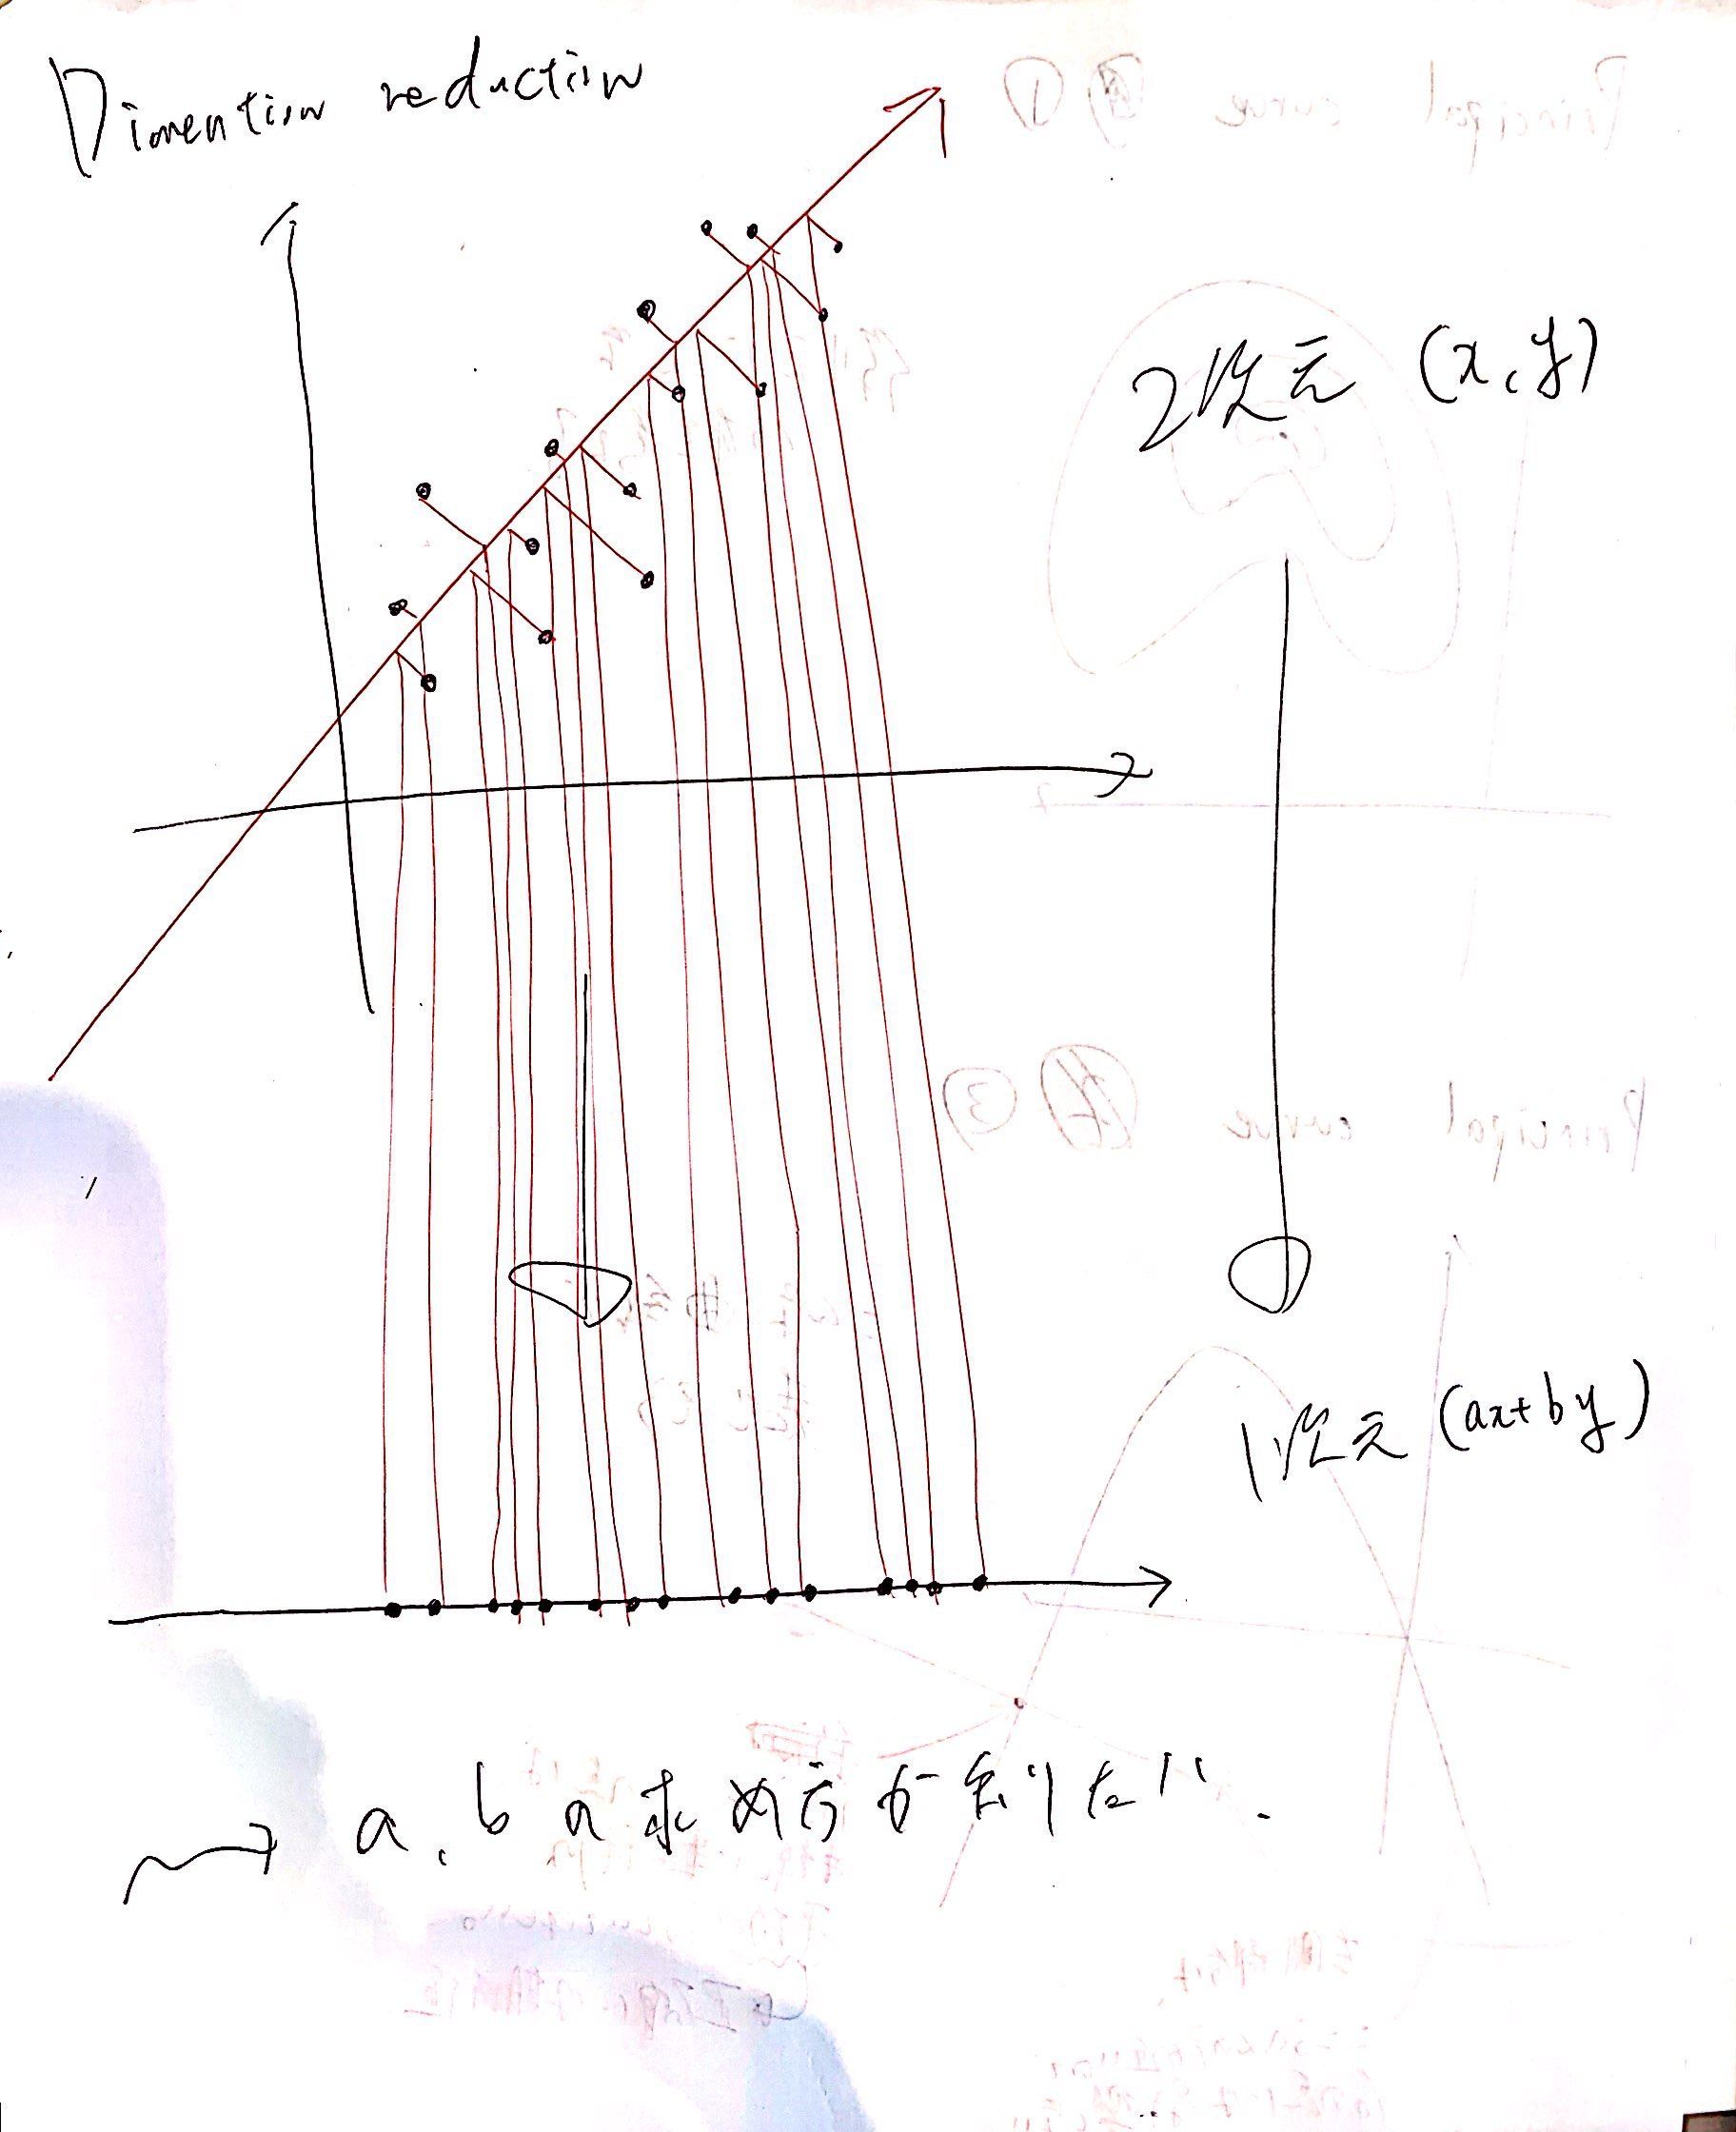
\includegraphics[width=5cm,clip]{images/dimention-reduction.jpg}
        \end{figure}
      \end{column}
    \end{columns}
  \end{frame}
  \begin{frame}{主成分分析}
    \begin{itemize}
      \item 主成分は, 一番単純な次元削減. 直線上に射影する.(下の画像のイメージ)\\
        \begin{figure}[htb]
          \centering
          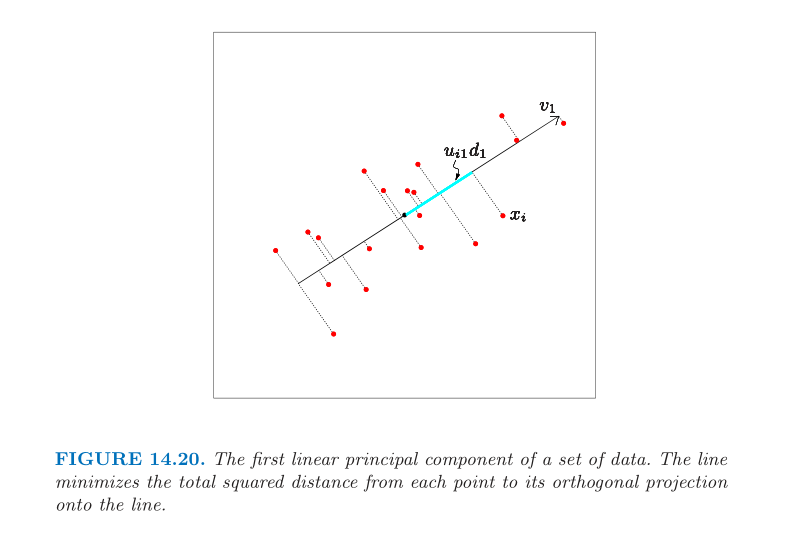
\includegraphics[width=4cm,clip]{images/pca.png}
        \end{figure}
      \item 直線は, 射影後のデータの分散が最大になるものを探す.
      \item 数式で書くと, 直交$p\times q$行列$\textbf{V}_q$で,
        \[
          \sum_{i=1}^N|(x_i-\bar{x})-\textbf{V}_q\textbf{V}_q^T(x_i-\bar{x})|^2
        \]
        を最小化するものを用いて, $X \to \textbf{V}_q\textbf{V}_q^TX$という変換で表せる.
      \item 行列の対角化や特異値分解で解ける. 深入りすると線形代数の沼. 時間が余ったら.
      \item 残差に対して主成分分析をすると, 第2主成分, 第3主成分, $\dots$と求まっていく.
      \item 参考\\
        \begin{enumerate}
          \item 主成分分析\\
            \url{https://blog2.cct-inc.co.jp/blog/machine-learning/pca_kaisetsu/}\\
          \item 線形代数\\
            \url{https://kriver-1.hatenablog.com/entry/2018/10/07/010758}
        \end{enumerate}
    \end{itemize}
  \end{frame}
  \begin{frame}{主曲線}
    主成分分析は, 直線や平面への射影を考えた. これを曲線や曲面への射影に応用する.

    まずは曲線版である主曲線(principal curve)について.
    分布に対する主曲線を考え, その後有限のデータセットに対する主曲線を考える.

    \begin{itemize}
      \item 分布に対する主曲線とは, 以下で定まる曲線.
      \[
        f(\lambda)=\mathrm{E}(X\mid \lambda_f(X)=\lambda)
      \]
      ただし, $\lambda_f$は入力変数の空間の各点に曲線$f_\lambda$上の最も近い点を対応付ける写像.
      次ページ以降の絵が分かりやすいと思う.
      \item 注意.\\
        一つの分布に対して, 主曲線は複数考えられることもある.
      \item 計算方法.\\
        期待値の計算と近傍の決定を繰り返す. (K平均法に似ている. alternating fashion.)\\
        \begin{figure}
          \centering
          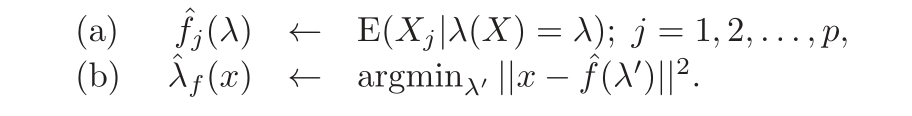
\includegraphics[width=8cm,clip]{images/principal.png}
        \end{figure}
      \item 曲線が近傍を決め, 近傍が曲線を決める. (self consistent)
    \end{itemize}
  \end{frame}
  \begin{frame}{分布に対する主曲線}
    \begin{figure}[htb]
      \centering
      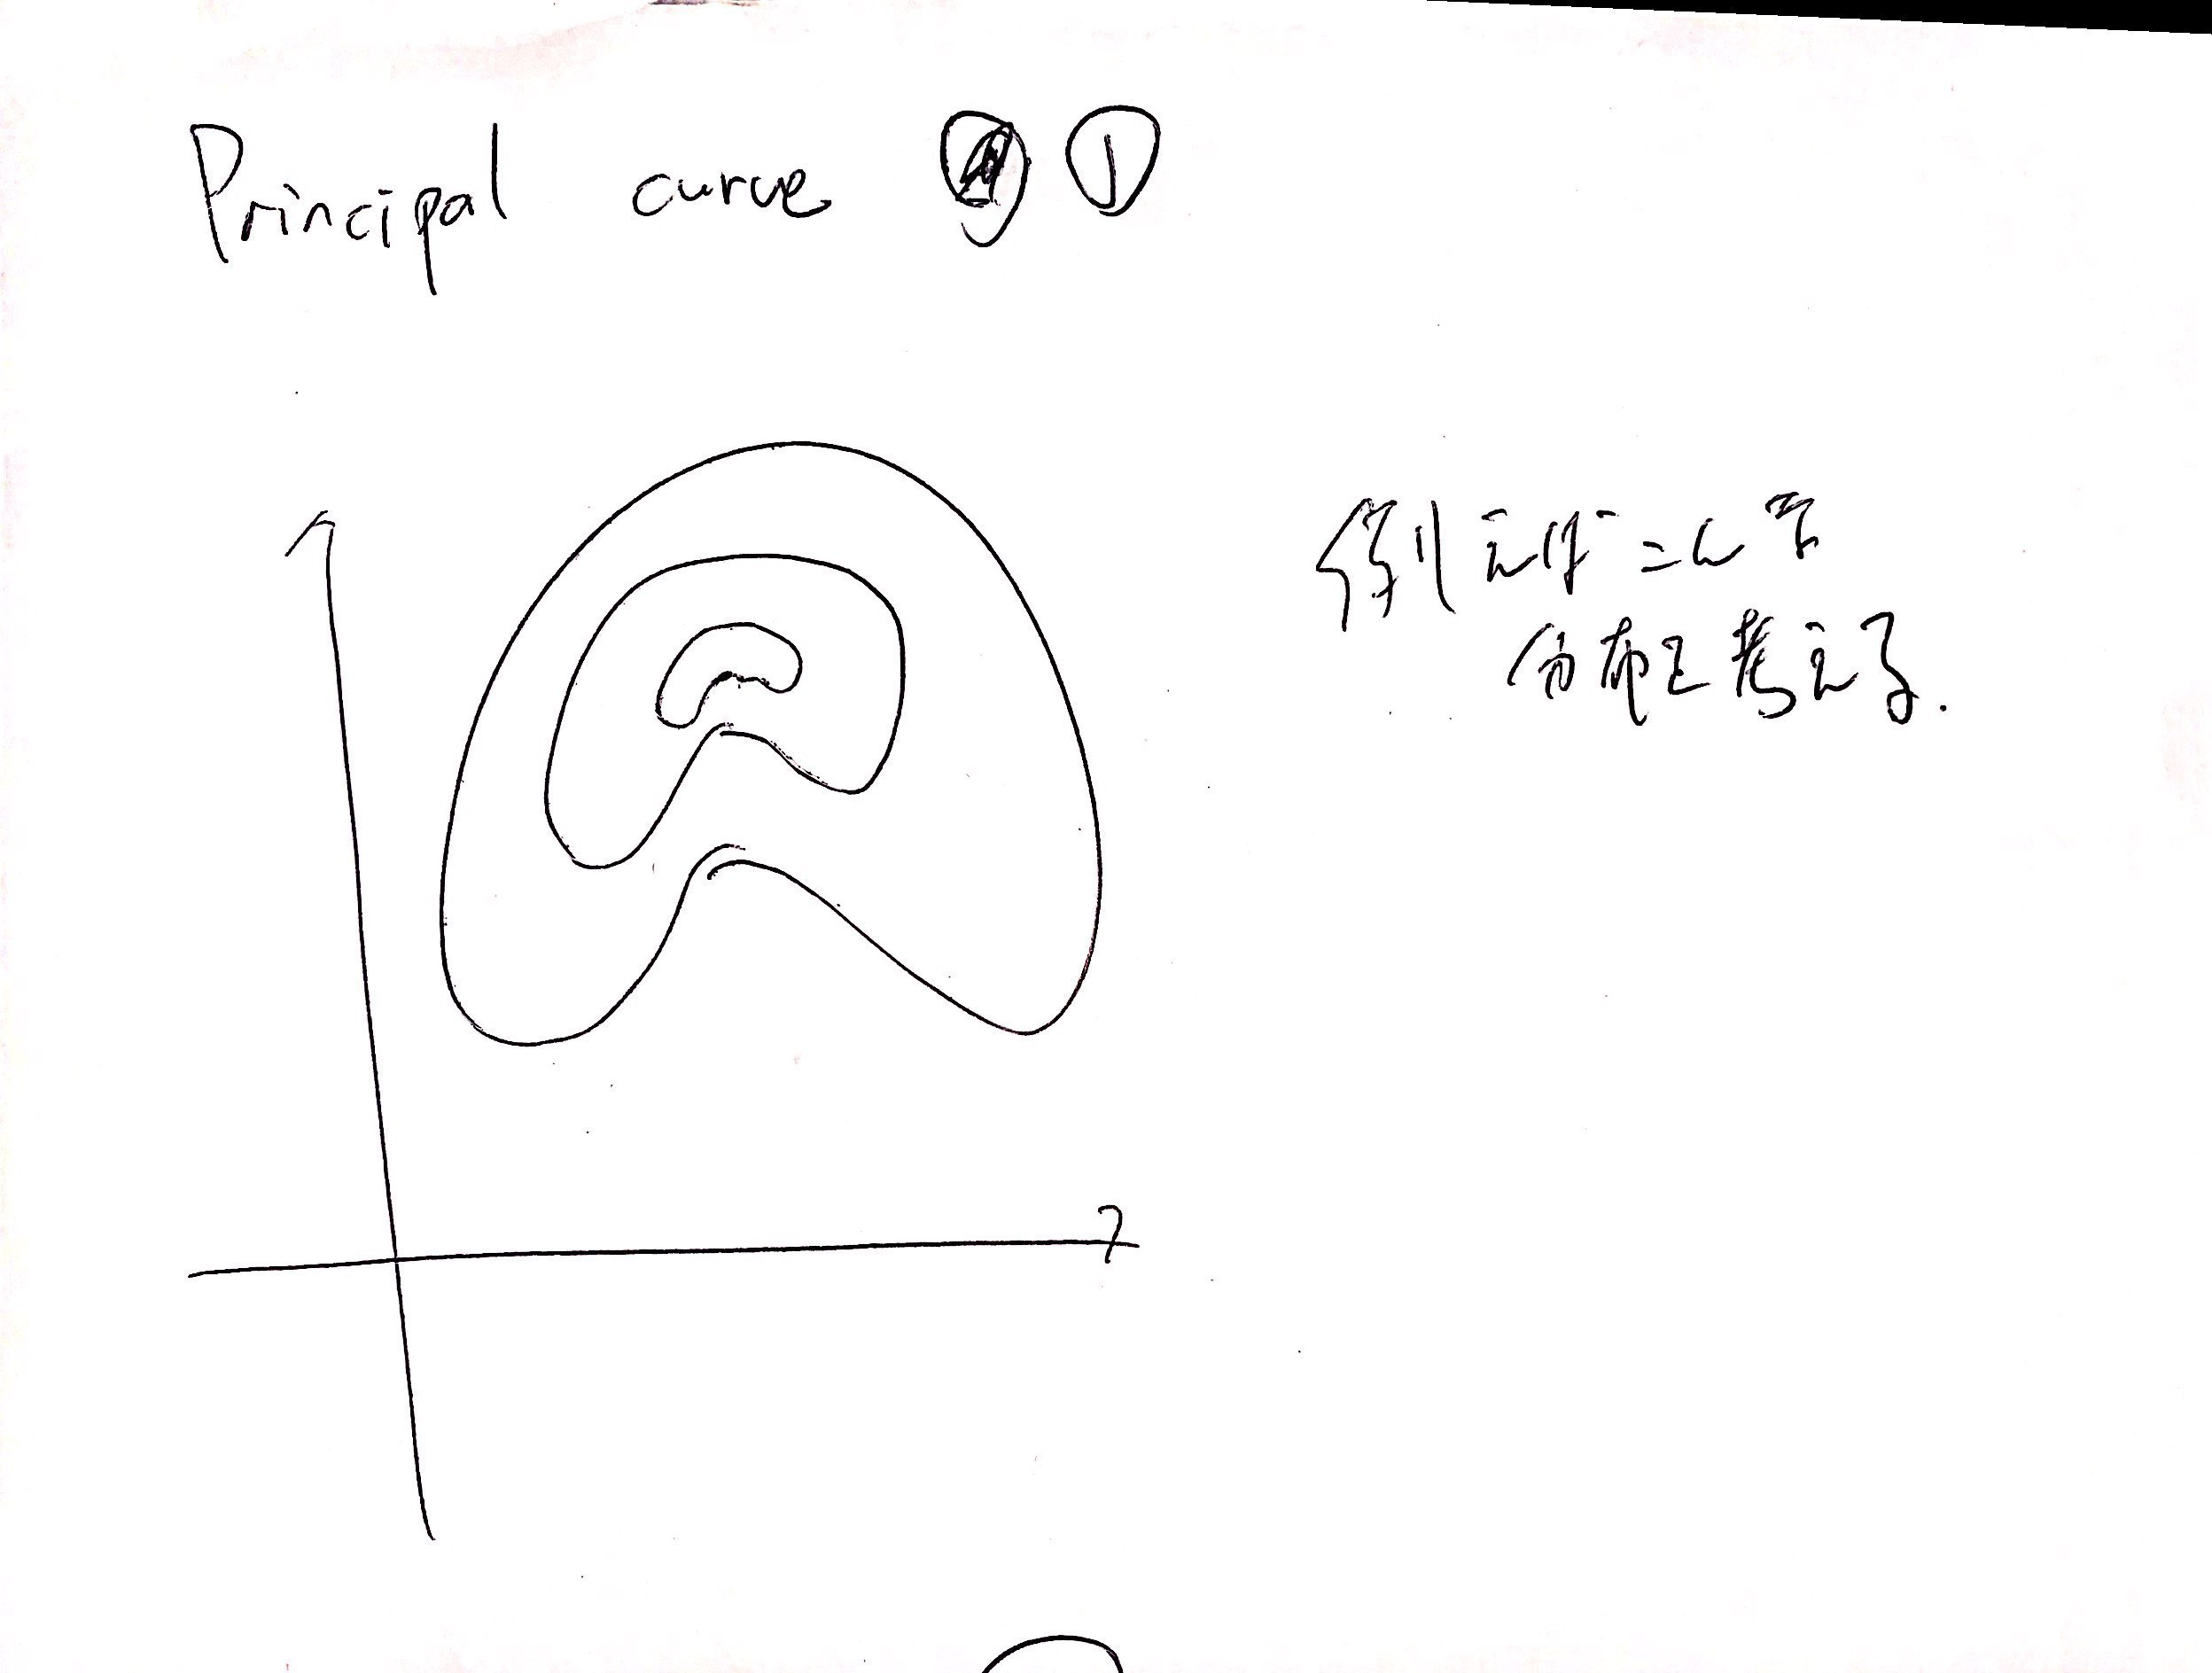
\includegraphics[width=10cm,clip]{images/principal-curve-distribution-1.jpg}
    \end{figure}
  \end{frame}
  \begin{frame}{分布に対する主曲線}
    \begin{figure}[htb]
      \centering
      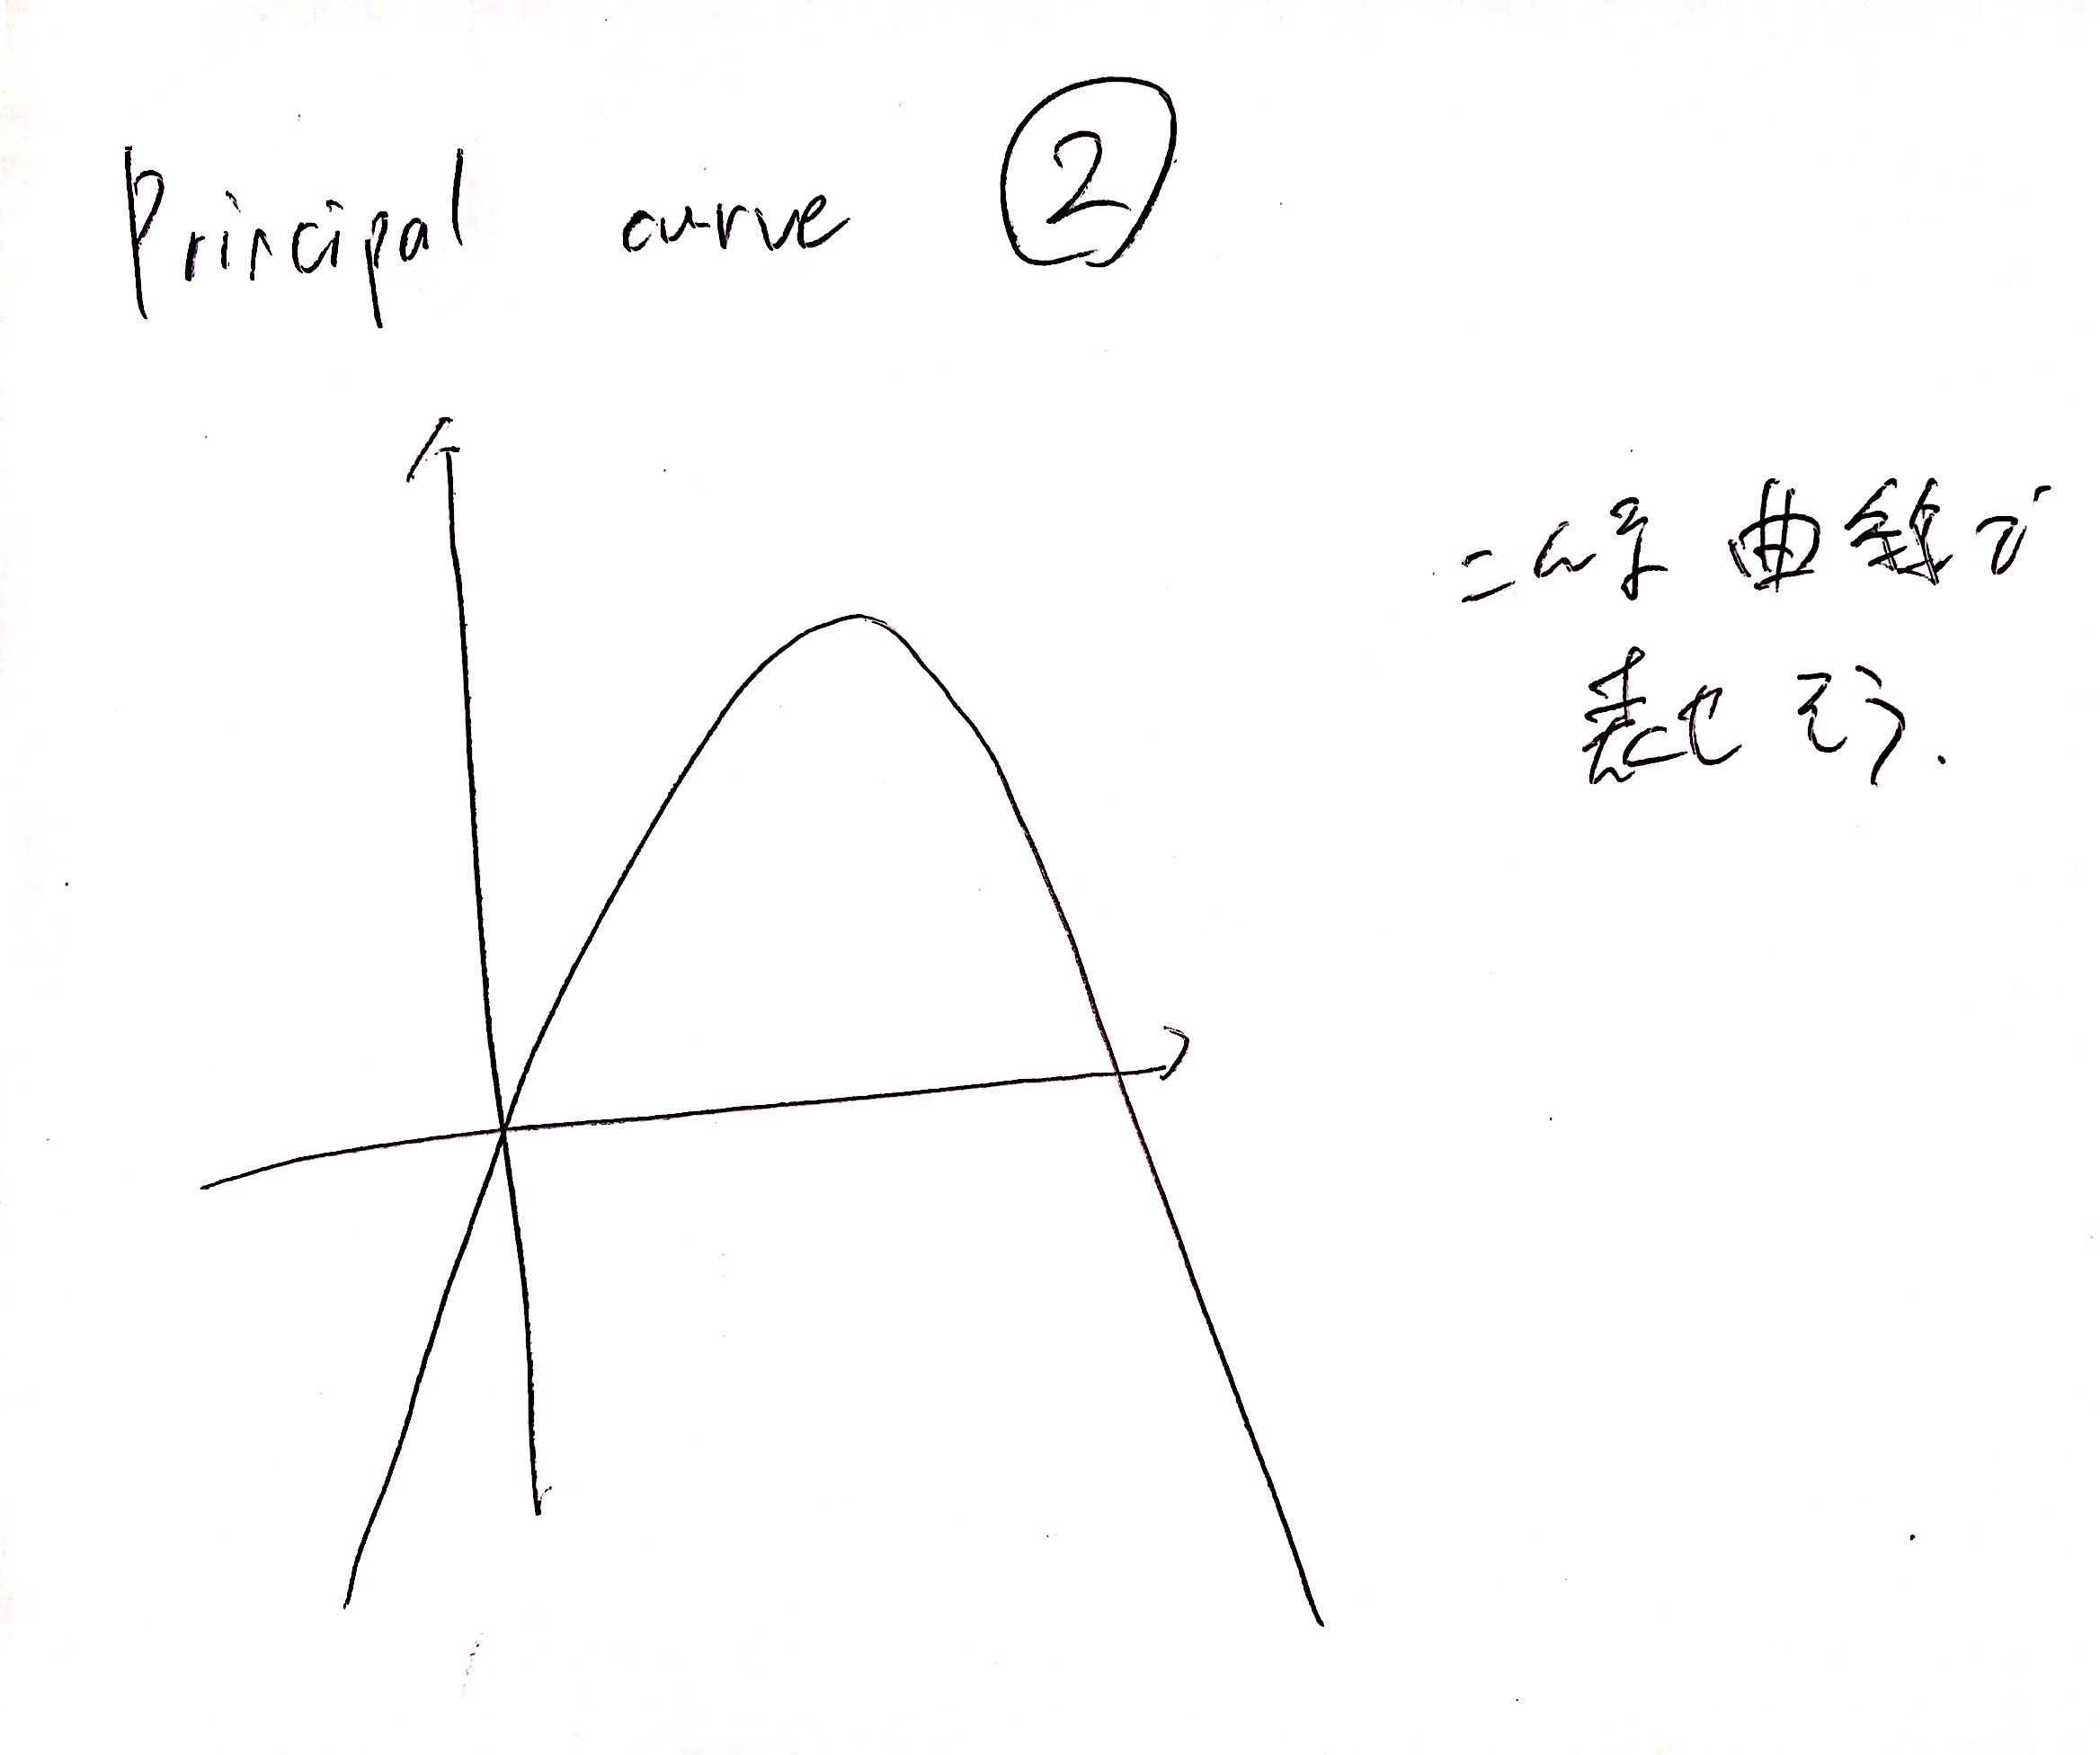
\includegraphics[width=10cm,clip]{images/principal-curve-distribution-2.jpg}
    \end{figure}
  \end{frame}
  \begin{frame}{分布に対する主曲線}
    \begin{figure}[htb]
      \centering
      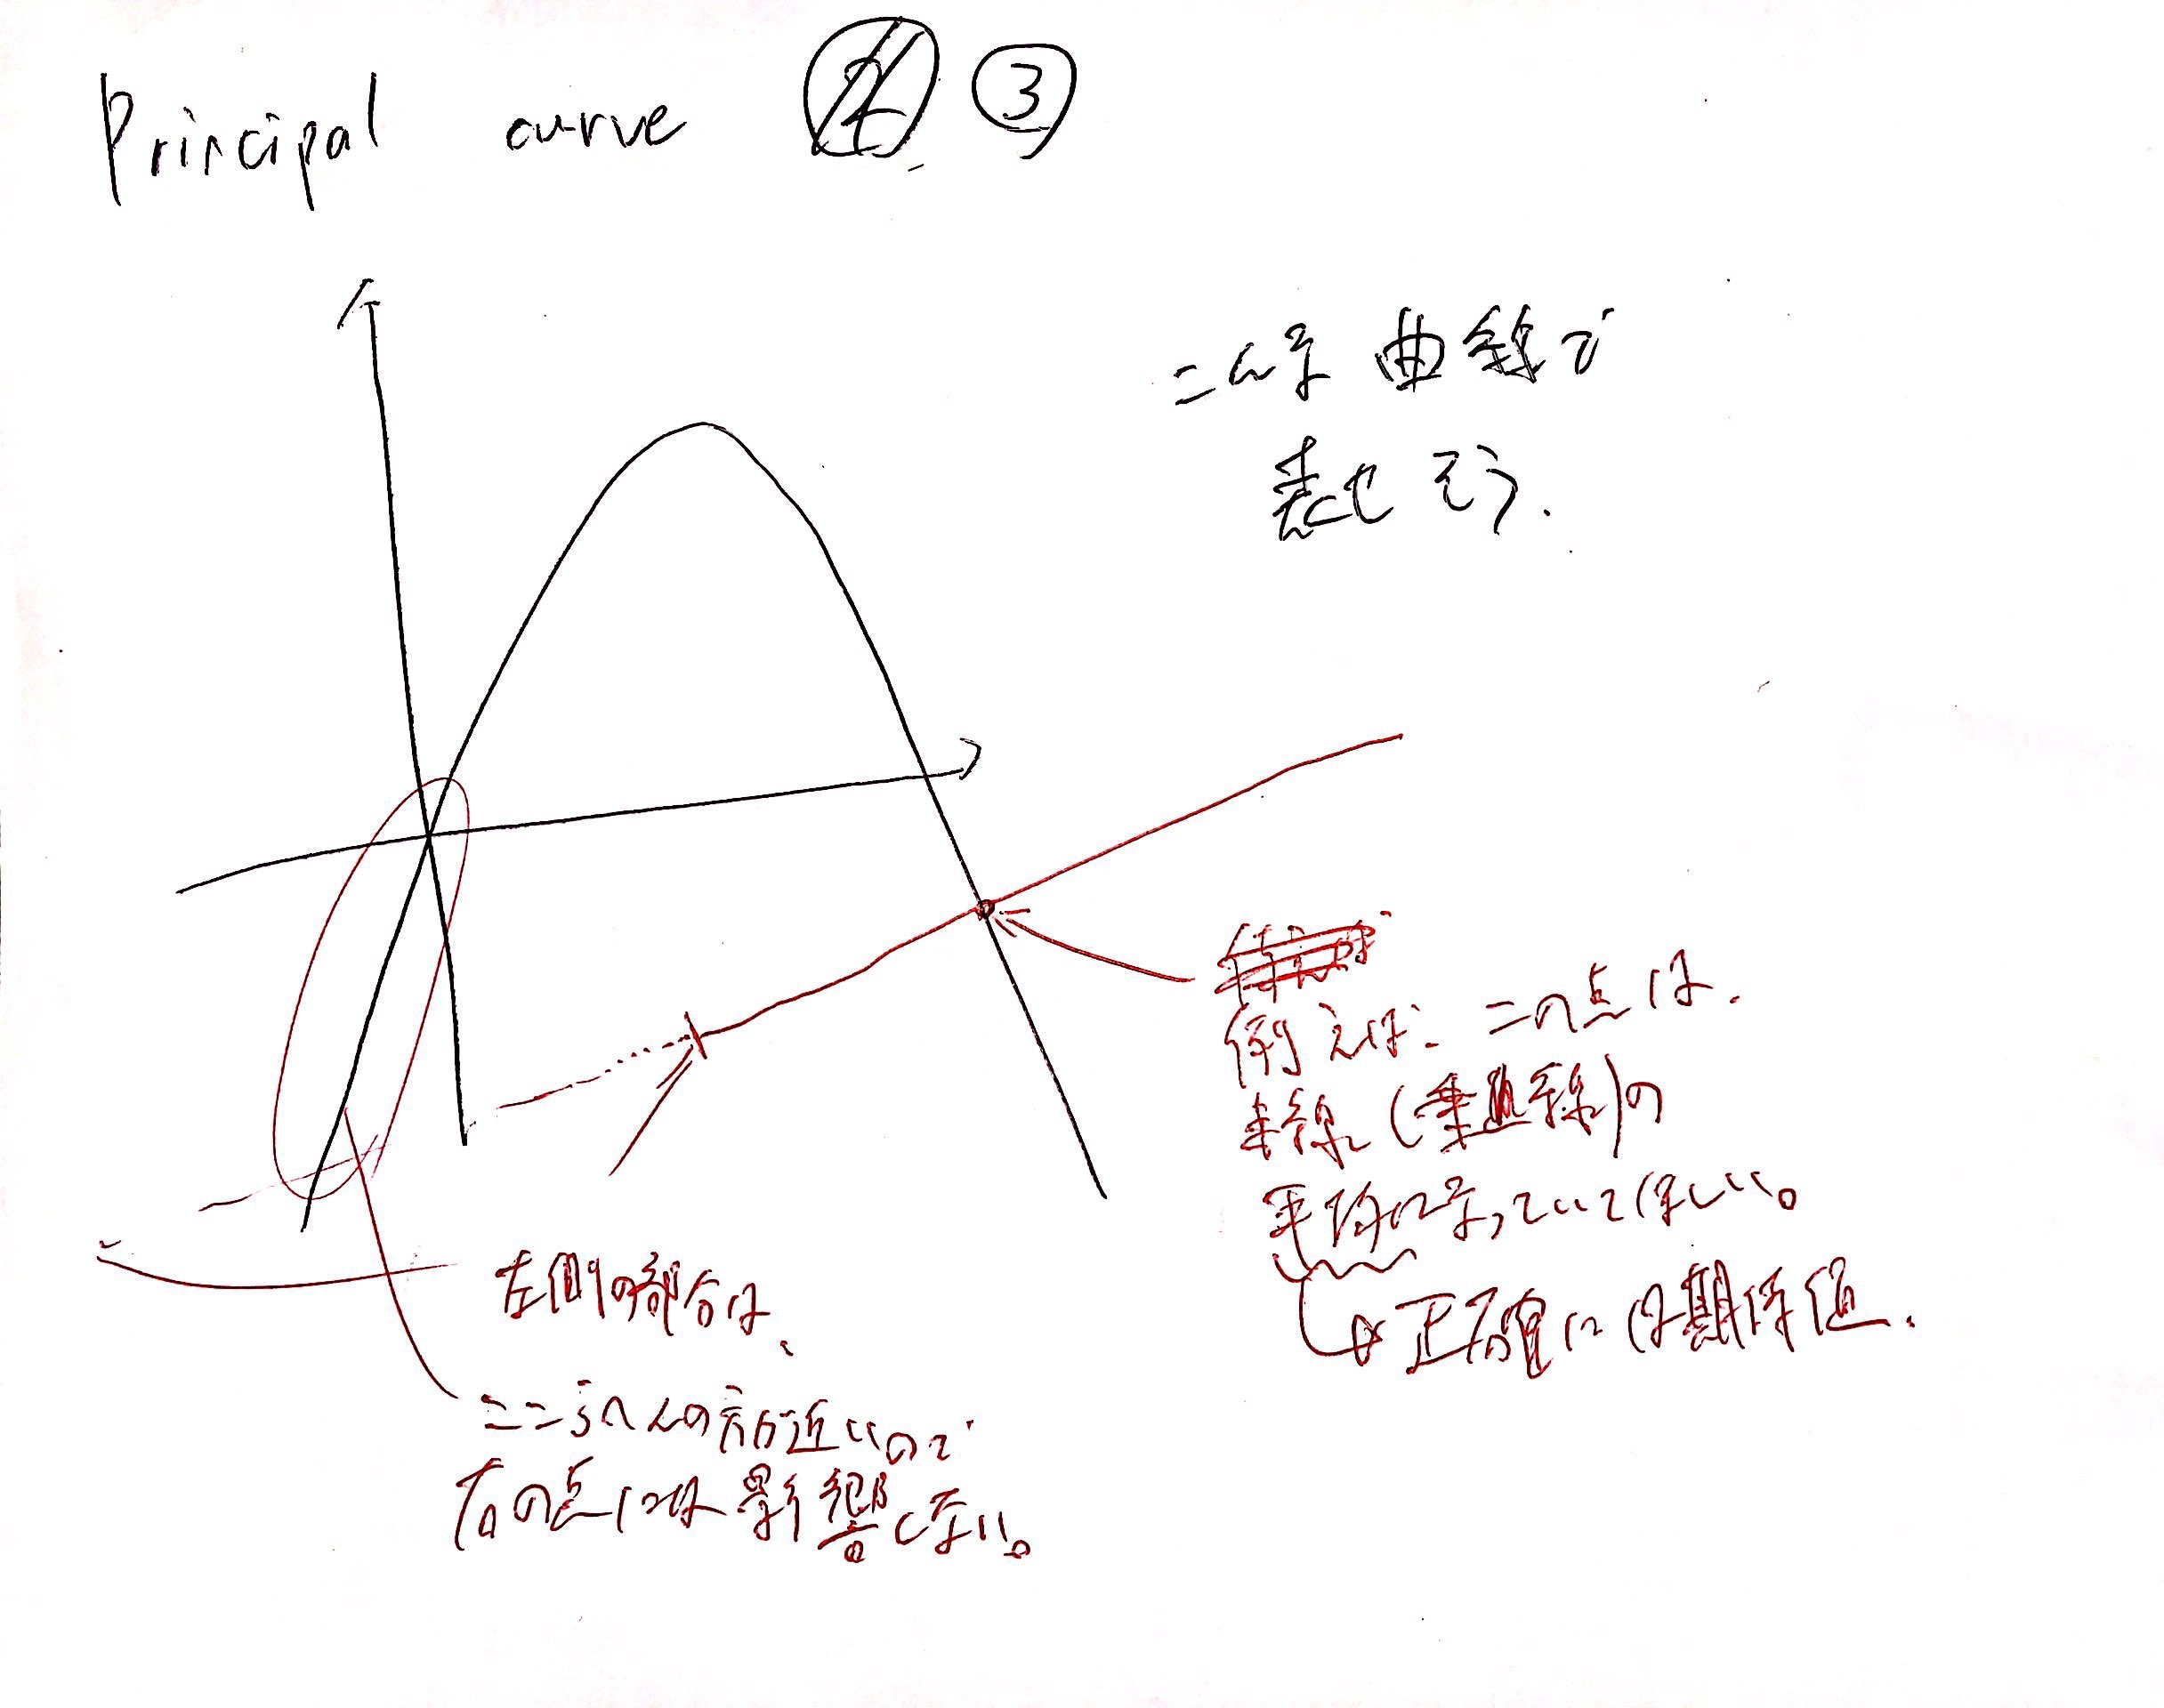
\includegraphics[width=10cm,clip]{images/principal-curve-distribution-3.jpg}
    \end{figure}
  \end{frame}
  \begin{frame}{データセットに対する主曲線}
    続いて, データセットに対する主曲線について.
    \begin{itemize}
      \item データセットに対する主曲線も基本的な考え方は一緒.
      \item ただ, 主曲線上の点で, 近傍にデータのない点が必ず存在してしまう.
      \item そこで, 期待値計算の時に``Scatterplot smoother''を使う.
      \item 主点(principal point)という概念も考えられる.
      これは, 任意個の点で各点がそれぞれのVoronoi領域の平均になっているもの.
      (self consistent)

      これの無限個バージョンが主曲線と思うこともできる.

      \item 主面(principal surface)は, 主曲線の2次元バージョン.
    \end{itemize}
  \end{frame}
  \begin{frame}{スペクトルクラスタリング}
    同心円みたいな, 通常の距離によるクラスタリングではうまくいかないケースのための方法.
    (同心円ってわかるなら, 教師あり学習では?subject matter consideration?)

    まずは計算方法から. 原理は後で.
    \begin{itemize}
      \item 類似度行列とは, $N\times N$行列で, $i$行$i'$列目の要素$s_{ii'}$は
        $i$個目と$i'$個目のデータの類似度を表す行列.
      \item 類似度の例としては, $x_i$と$x_{i'}$のユークリッド距離を$d_{ii'}$として,
        $s_{ii'}=\exp(\frac{-d_{ii'}^2}{c})$とする方法がある. $c$はパラメータ.
      \item 類似度行列とから重み付きの無向グラフを作る.
        基本的に, 各ノードは訓練データに対応し, 各辺には, 類似度の重みがついているとすればよい.
      \item グラフの定め方にはいくつかの方法がある. 例えば, 各ノードの$K$近傍を考え,
        \[
          w_{ii'}=
          \begin{cases}
            s_{ii'} \quad \mbox{if} x_i, x_{i'}\mbox{は互いに互いの}K\mbox{近傍に入っている}\\
            0 \quad \mbox{otherwise}
          \end{cases}
        \]
        としてもよい.
      \item グラフの重みに関しても, $N$次正方行列$\textbf{W}=\{w_{ii'}\}$が作れる. 隣接行列.
      \item 隣接行列から次数行列$\textbf{G}$を作れる.
        \[
          \textbf{G}=\mathrm{diag}\left(g_i=\sum_{j=1}^Nw_{ij}\right)
        \]
    \item さらに, unnormalized graph laplacian$\textbf{L}$を
      \[
        \textbf{L}=\textbf{G}-\textbf{W}
      \]
      で定める.

    \end{itemize}
  \end{frame}
  \begin{frame}{スペクトルクラスタリング}
    \begin{itemize}
      \item $\textbf{L}$を対角化し, 固有値の小さい方から$m$個に対応する固有ベクトルを並べて,
        $N\times m$行列$\textbf{Z}$を作る.
      \item $\textbf{Z}$の行ベクトルを, K平均法などでクラスタリングする.
    \end{itemize}
    以上が, スペクトルクラスタリングの流れ. なんでうまくいくのか意味不明だと思うので, 以下, 数学的な背景の説明.
    \begin{itemize}
      \item まず, 任意のベクトル$\textbf{f}$について,
        \begin{eqnarray*}
          \textbf{f}^T\textbf{L}\textbf{f}&=\sum_{i=1}^Ng_if_i^2-\sum_{i=1}^N\sum_{i'=1}^Nf_if_{i'}w_{ii'}\\
          &=\frac{1}{2}\sum_{i'=1}^Nf_if_{i'}w_{ii'}(f_i-f_{i'})^2
        \end{eqnarray*}
        が成り立つ.
      \item この値が小さくなるのは, ``$w_{ii'}$が大きいならば, $f_i$と$f_{i'}$の値が近い''時である.
      \item さらに言うと, $1^T\textbf{L}1=0$であるので, 定数ベクトルは固有値$0$に対応する固有ベクトル.
        グラフが完全にクラスターで分離していれば, $\textbf{L}$はブロック対角行列になるので,
        クラスター$G$に対して, ベクトル$I_G$も固有値0に対応する固有ベクトルとなる.
    \end{itemize}

    参考
    \url{https://techblog.nhn-techorus.com/archives/5464}
  \end{frame}
  \begin{frame}{カーネル主成分}
    普通の主成分の非線形化バージョン.

    普通の主成分は, 分散行列の対角化として得られる.
    数式で書くと, $\textbf{X}$のグラム行列
    \[
      \textbf{K}=\textbf{X}\textbf{X}^T
    \]
    の二重中心化行列の対角化
    \[
      \tilde{\textbf{K}}=(\textbf{I}-\textbf{M})\textbf{K}(\textbf{I}-\textbf{M})=\textbf{U}\textbf{D}^2\textbf{U}^T
    \]
    を考えることである. 詳細は18章にて.

    カーネル主成分分析は, 上のグラム行列$K$の代わりに,
    カーネル行列$\{K(x_i,x_{i'})\}$を取ったもの.
    カーネル行列の各成分は, 内積$\varphi(x_i)\cdot\varphi(x_{i'})$である.
    イメージとしては, 高次元に射影して, 普通の主成分分析をしている.

    この続き, カーネル主成分の別視点からの理解.
    再生核ヒルベルト空間の話. パス.
  \end{frame}
  \begin{frame}{疎な主成分}
    主成分は, どの変数が寄与度が高いかを教えてくれる. \\
    →主成分が疎(sparce)だと嬉しい. \\
    →疎な主成分を得る方法について. 正規化条件を加えて, 最適化する.
    最適化のアプローチは大きく2種類. とりあえず, 正規化はlassoを考える.
    \begin{itemize}
      \item 分散を最大化する.
        \[
          \mathrm{maximize} \quad v^T(\textbf{X}^T\textbf{X})v \quad \mathrm(subject to) \quad \sum_{j=1}^p|v_j| \le t, v^Tv=1
        \]
      \item 正規化項を加えた損失を最小化する.
        \[
          \mathrm{minimize} \quad \sum_{i=1}^N|x_i-\theta v^Tx_i|_2^2+\lambda|v|_2^2+\lambda_1|v|_1 \quad \mathrm{subject to} \quad |\theta|_2=1
        \]
        この式について考察.
        \begin{itemize}
          \item $\lambda=\lambda_1=0$のとき, これは通常の主成分で, $\theta=v$
          \item $p \gg N$のとき, 最適解が一意に定まらないことがある
          \item 第3項が疎にするための制約
        \end{itemize}
    \end{itemize}
  \end{frame}
  \section{非負行列因子分解\\p.553-}
  \begin{frame}{非負行列因子分解の概要}
    主成分分析の代案となる次元削減の方法として, 最近(1999)提案された手法. \\
    データや主成分の値が非負であるときに使える. 画像データなどが典型.

    主となる式は, 以下. 確かに次元削減できている.
    \begin{figure}[htb]
      \centering
      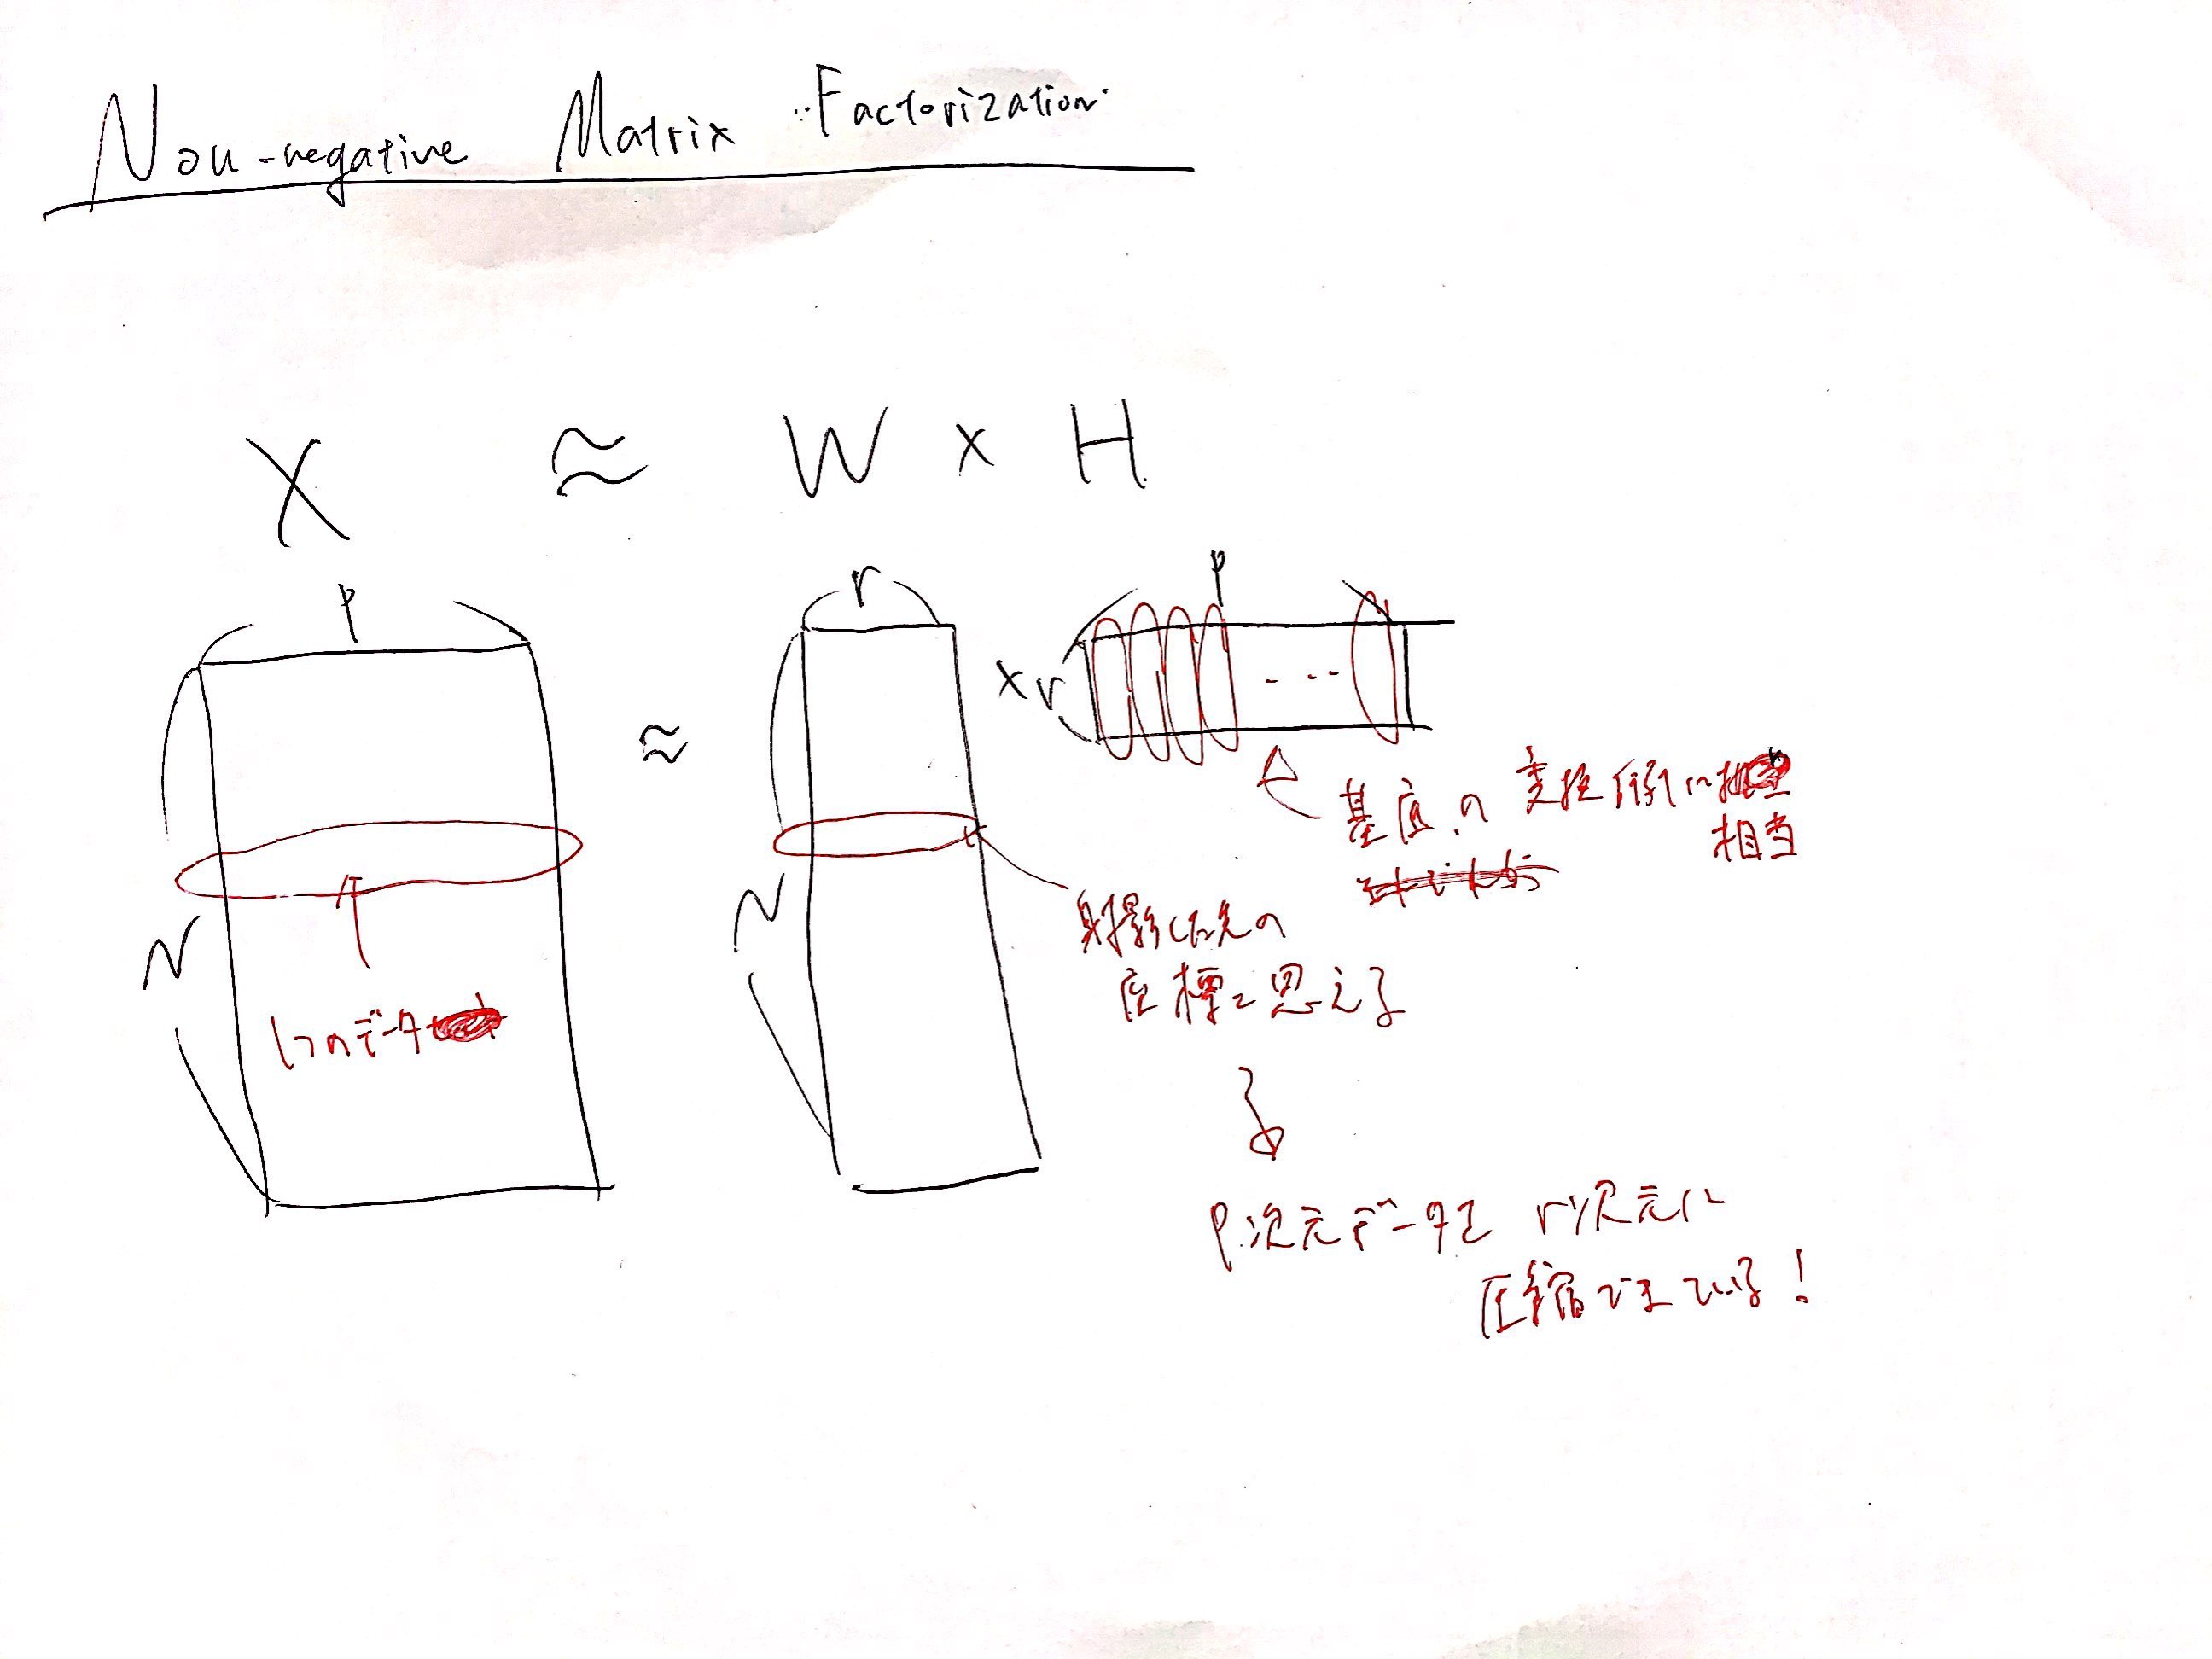
\includegraphics[width=7cm,clip]{images/nmf-overview.jpg}
    \end{figure}
  \end{frame}
  \begin{frame}{非負行列因子分解の計算}
    前頁の$\textbf{W}$, $\textbf{H}$は以下の最大化で求める.
    \[
      L(\textbf{W}, \textbf{H})=\sum_{i=1}^N\sum_{j=1}^p\left(x_{ij}\log(\textbf{WH})_{ij}-(\textbf{WH})_{ij}\right)
    \]
    これは, 各変数$X_i$がPoisson分布としたときの対数尤度.
    非負データに対して, Poisson分布を仮定するのは妥当とのこと.

    以下のアルゴリズムで近似できる. (alternating fashion)\\
    上の尤度の偏微分$=0$という意味.
    \begin{figure}[htb]
      \centering
      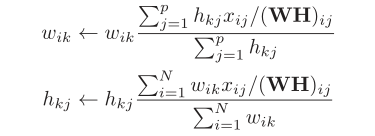
\includegraphics[width=5cm,clip]{images/nnmf.png}
    \end{figure}
  \end{frame}
  \begin{frame}{非負行列因子分解の問題点}
    問題点として, 行列の分解が一意でないことが挙げられる. \\
    これに対する解決策は記述なし.
    そんなに気にせず(結構)使われているっぽい.
    \begin{figure}[htb]
      \centering
      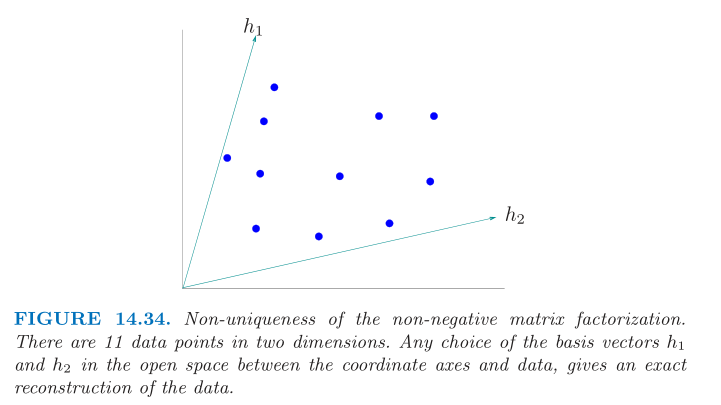
\includegraphics[width=7cm,clip]{images/nnmf-nonuniqueness.png}
    \end{figure}
    上の画像は一意に決まらない例.
    2次元→2次元の分解とすると, 実質軸の回転と思える.

    →値が非負を保つ軸の回転って, いくらでもあるよね.
  \end{frame}
  \begin{frame}{原型分析}
    非負行列因子分解と似た, K平均法と似た発想の手法. \\
    \begin{figure}[htb]
      \centering
      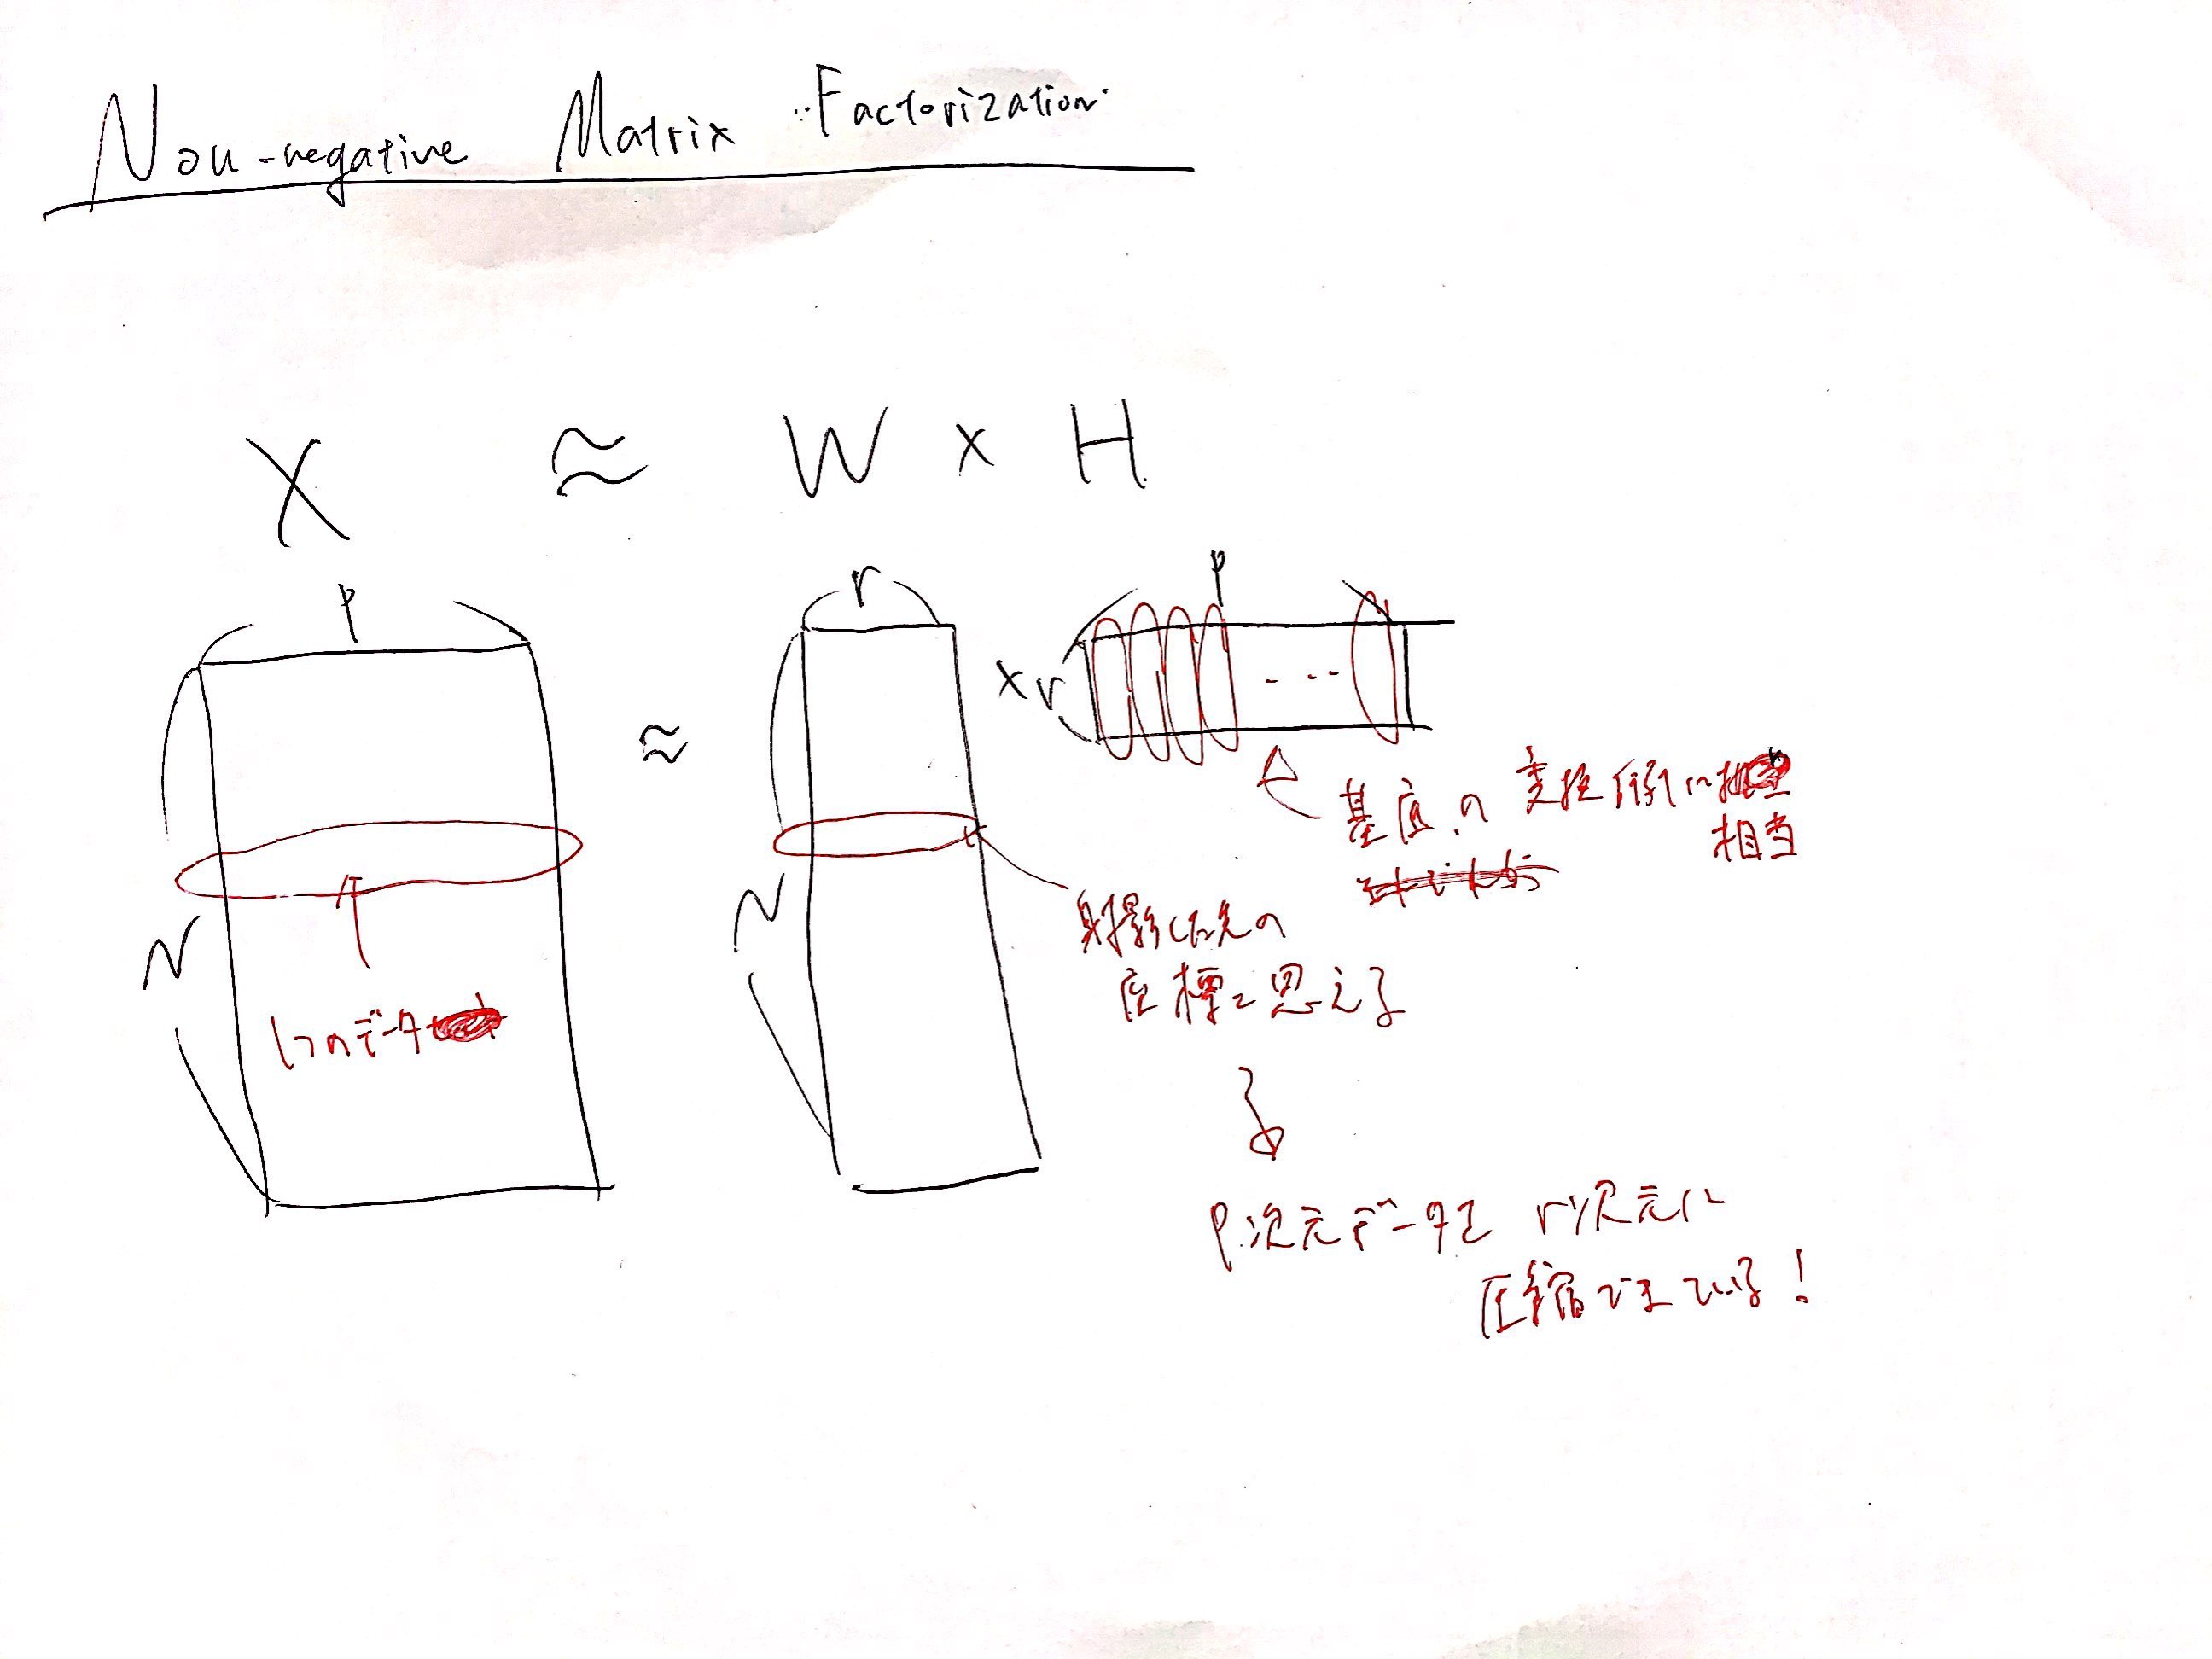
\includegraphics[width=5cm,clip]{images/nmf-overview.jpg}
    \end{figure}
    ここまでは一緒. 最適化する式が違う.
  \end{frame}
  \begin{frame}{原型分析の計算}
    \[
      \textbf{H}=\textbf{BX}
    \]
    を満たす行列$\textbf{B}$で, $\sum_k{b_{ik}}=1$を満たすものが取れる.
    これらを使って, 以下を最小化する.
    \[
      J(\textbf{W},\textbf{B})=|\textbf{X}-\textbf{WH}|^2=|\textbf{X}-\textbf{WBX}|^2
    \]
    計算は, 今まで見たいに, 交互に代入していけば, 最適解を求められる. (alternating fashion)
    \begin{itemize}
      \item データを代表点の凸結合で表すだけでなく, 代表点をデータの凸結合で表していると思える.
      \item 前者の凸結合が1個の代表点だけからなり, 後者の凸結合が平均であるものがK平均法と思える.
    \end{itemize}
  \end{frame}
  \begin{frame}{非負行列因子分解と原型分析}
    この2つ, 式の形は似ているが, 使われる目的は異なる.
    \begin{itemize}
      \item 非負行列因子分解

        各変数の分布をより少ない変数で表したい. \\
        →$\textbf{X}$の各列をうまく近似しようとする.

      \item 原型分析

        各データをより少ない次元でうまく表現したい. \\
        →$\textbf{X}$の各行をうまく近似しようとする.
    \end{itemize}
  \end{frame}
  \section{独立成分分析と探索的射影追跡\\p.557-}
  \begin{frame}{潜在変数と因子分析}
    実際問題, 測れてるデータって, 本当に測りたいおおもとのデータじゃないこと多いよね. \\
    (例えば, 大学入試は学力を測りたいから各教科の試験を受けさせる)\\
    →計測した変数の背後にある``本質的な''パラメータ(=潜在変数, latent variables)を測りたい. \\
    →因子分析(factor analysis)の出番.
    \begin{figure}[htb]
      \centering
      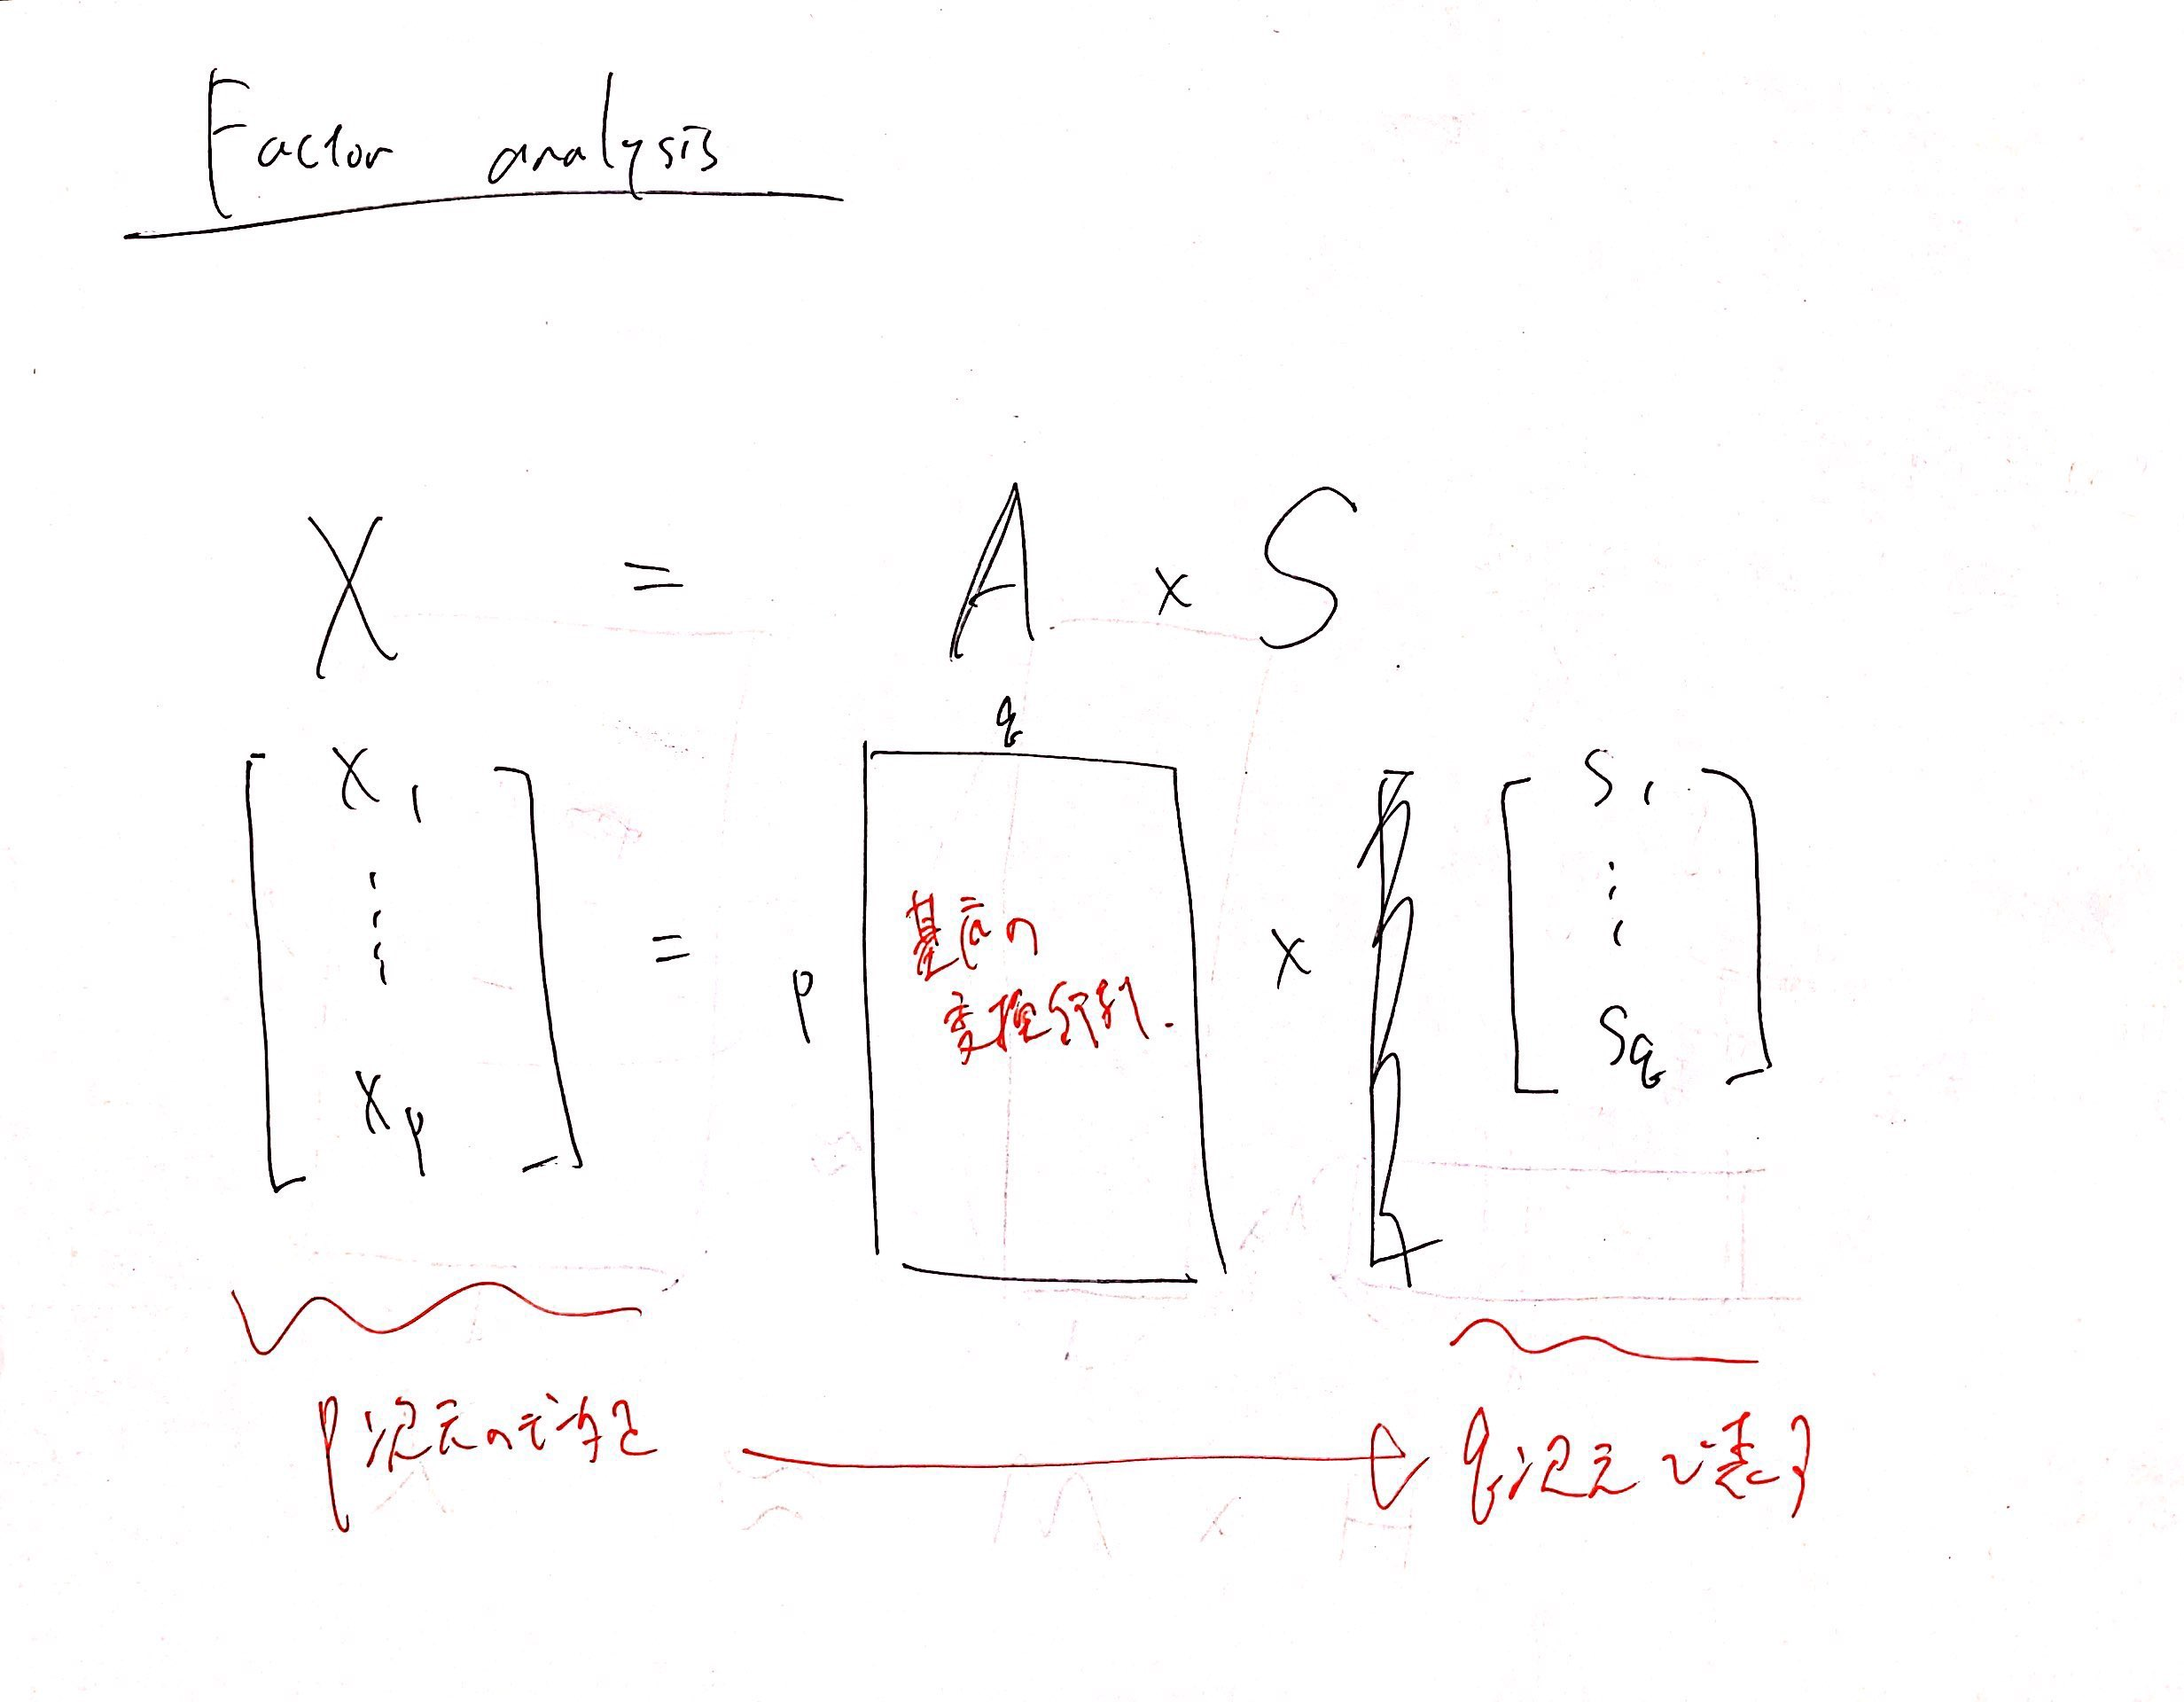
\includegraphics[width=7cm,clip]{images/fa-overview.jpg}
    \end{figure}
  \end{frame}
  \begin{frame}{因子分析}

    計算は以下の手順で進む.
    \begin{itemize}
      \item 変数空間の中で, 情報量の多い部分空間を見つける. (次元削減と同義. 主成分分析. )
      \item 見つけた空間の中で, 適切な基底を見つける. (この操作を``回転''という. )
    \end{itemize}

    問題点がある.

    任意の直交行列$\textbf{R}$について,
    $X=\textbf{A}S=\textbf{A}\textbf{R}^T\textbf{R}S=\textbf{A}^*S^*$
    となるので, 潜在変数や係数行列の取り方は一意でない. (というか無限個ある. )\\
    →結局, どんな基底を取るか恣意的に決められてしまうので, 批判されている.

    \url{https://kayakura.me/factor-analysis/}
  \end{frame}
  \begin{frame}{独立成分分析}
    因子分析と式の形は完全に一緒.
    \[
      X=\textbf{A}S
    \]

    $S$の各変数が無相関なだけでなく, 統計的に独立であることを要求することで, 回転による恣意性を克服している. \\
    (無相関は二次のクロスモーメントが0, 独立性は全てのクロスモーメントが0という要求. )\\
    →分解が一意に定まる. (ただし, 多変量ガウス分布は例外らしい.(?))
  \end{frame}
  \begin{frame}{独立成分分析の計算}
    独立性が重要なので, 少しでも独立具合の高い基底をとりたい. \\
    →結論, 因子分析の回転の基準が``独立度''に設定された, と思ってよい.

    以下, 独立度の測り方について.
    情報理論の話.\\
    \url{https://logics-of-blue.com/information-theory-basic/}

    分布$g(y)$に従う変数$Y$のエントロピー$H(Y)$は,
    \[
      H(Y)=-\int g(y)\log g(y)\mathrm{d}y
    \]
    で定まる. さらに, $Y$の相互情報量$I(Y)$が
    \[
      I(Y)=\sum_{j=1}^pH(Y_j)-H(Y)
    \]
    で定まる. これは, Kullback-Leibler距離とも呼ばれ,
    分布$g(y)$と独立な分布$\prod_jg_j(y_j)$の間の距離を表す.

    →相互情報量が大きいほど独立度が低いということ.

  \end{frame}
  \begin{frame}{独立成分分析の計算}
    相互情報量が, いい感じに独立度を定式化できているので, 採用.

    $Y$が$X$の回転と思う. すなわち, $Y=\textbf{A}^TX$.
    すると,
    \[
      I(Y)=\sum_{j=1}^pH(Y_j)-H(\textbf{A}^TX)=\sum_{j=1}^pH(Y_j)-H(X)
    \]
    となる.

    情報理論で, ガウス分布はエントロピー最大と知られている.
    やりたいことは, 独立度最大化=相互情報量最小化=ガウス分布からできるだけ遠ざける, と思える.

    (実際には, エントロピーでないものを使ったりするらしいのだが, 情報理論に深入りしていきそうなので, パス)
  \end{frame}
  \begin{frame}{探索的射影追跡}
    データを低次元に射影するときに, どの軸を取るといいかな?という話.\\
    →興味のある軸はガウス分布から遠い軸.\\
    (中心極限定理. 分離できていないと, ガウス分布になっちゃう. って話なのだろうか. )
    →結局やるのは, エントロピーとかを使った計算.\\
    →計算は, 独立成分分析と似た感じになるよ.

  \end{frame}
  \begin{frame}{独立成分分析を直接計算する}
    \begin{itemize}
      \item 回転とかせずに, 直接独立成分を求めたい.
      \item 独立性から, 混合分布はただの積.
        \[
          f_S(s)=\prod_jf_j(s_j)
        \]
      \item ``独立である$fallingdotseq$ガウス分布と遠い''という話を思い出す.\\
        →ガウス分布からの乖離具合が表現できるように定式化.
        \[
          f_j(s_j)=\phi(s_j)e^{g_j(s_j)}
        \]
      \item ここまではやりたいことが分かった. 続きが分からなかった.
      \item 以下を最大化.
        \begin{figure}[htb]
          \centering
          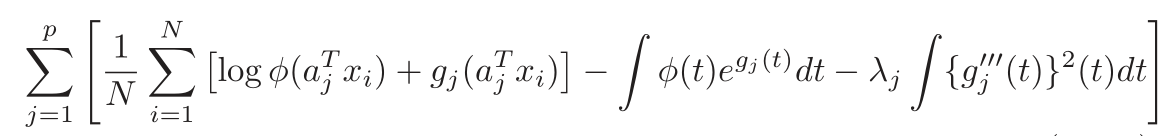
\includegraphics[width=10cm,clip]{images/prodenica.png}
        \end{figure}
        \begin{itemize}
          \item 第1項は対数尤度
          \item 第2項で正規化しているらしい. (?)
          \item 第3項はSmoother. 2次Splineを要求している. (?)
        \end{itemize}
    \end{itemize}
  \end{frame}
  \section{多次元尺度構成法\\p.570-}
  \begin{frame}{多次元尺度構成法(Multidimentional scaling)}
    \begin{itemize}
      \item 低次元で表現したい, というのはここまでと一緒. アプローチが違う.
      \item 各点の情報は使わず, 点間の非類似度$\fallingdotseq$距離$d_{ii'}$を使う.
      \item より低次元な空間の点の集合$z_1,\dots,z_N$で, ``距離''をうまく再現したものを探す.
      \item 例えばKruskal-Shephardスケーリングでは以下の``ストレス関数''を最小化する.
        \[
          S_M(z_1,\dots,z_N)=\sum_{i\ne i'}(d_{ii'}-|z_i-z_{i'}|)^2
        \]
      \item ストレス関数はほかにも.
        \begin{itemize}
          \item Sammon mapping: 近いものを再現することを重視する.
            \[
              S_{Sm}(z_1,\dots,Z_N) = \sum_{i\ne i'}\frac{(d_{ii'}-|z_i-z_{i'}|)^2}{d_{ii'}}
            \]
          \item Classical scaling: 類似度を使う.
            \[
              S_C(z_1,\dots,Z_N) = \sum_{i,i'}(s_{ii'}-(z_i-\bar{z}) \dot (z_{i'}-\bar{z}))
            \]
          \item Kruskal-Shephard nonmetric scaling: 非量的変数に対して使える.
            \[
              S_{NM}(z_1,\dots,Z_N) = \frac{\sum_{i\ne i'}(|z_i-z_{i'}|-\theta(d_{ii'}))^2}{\sum_{i\ne i'}|z_i-z_{i'}|^2}
            \]
        \end{itemize}
    \end{itemize}
  \end{frame}
  \begin{frame}{多次元尺度構成法の強み}
    \begin{itemize}
      \item PCAやSOMは, 近い点の近さは保つ一方, 遠い点を近くしてしまうかもしれない.
        \begin{figure}
          \centering
          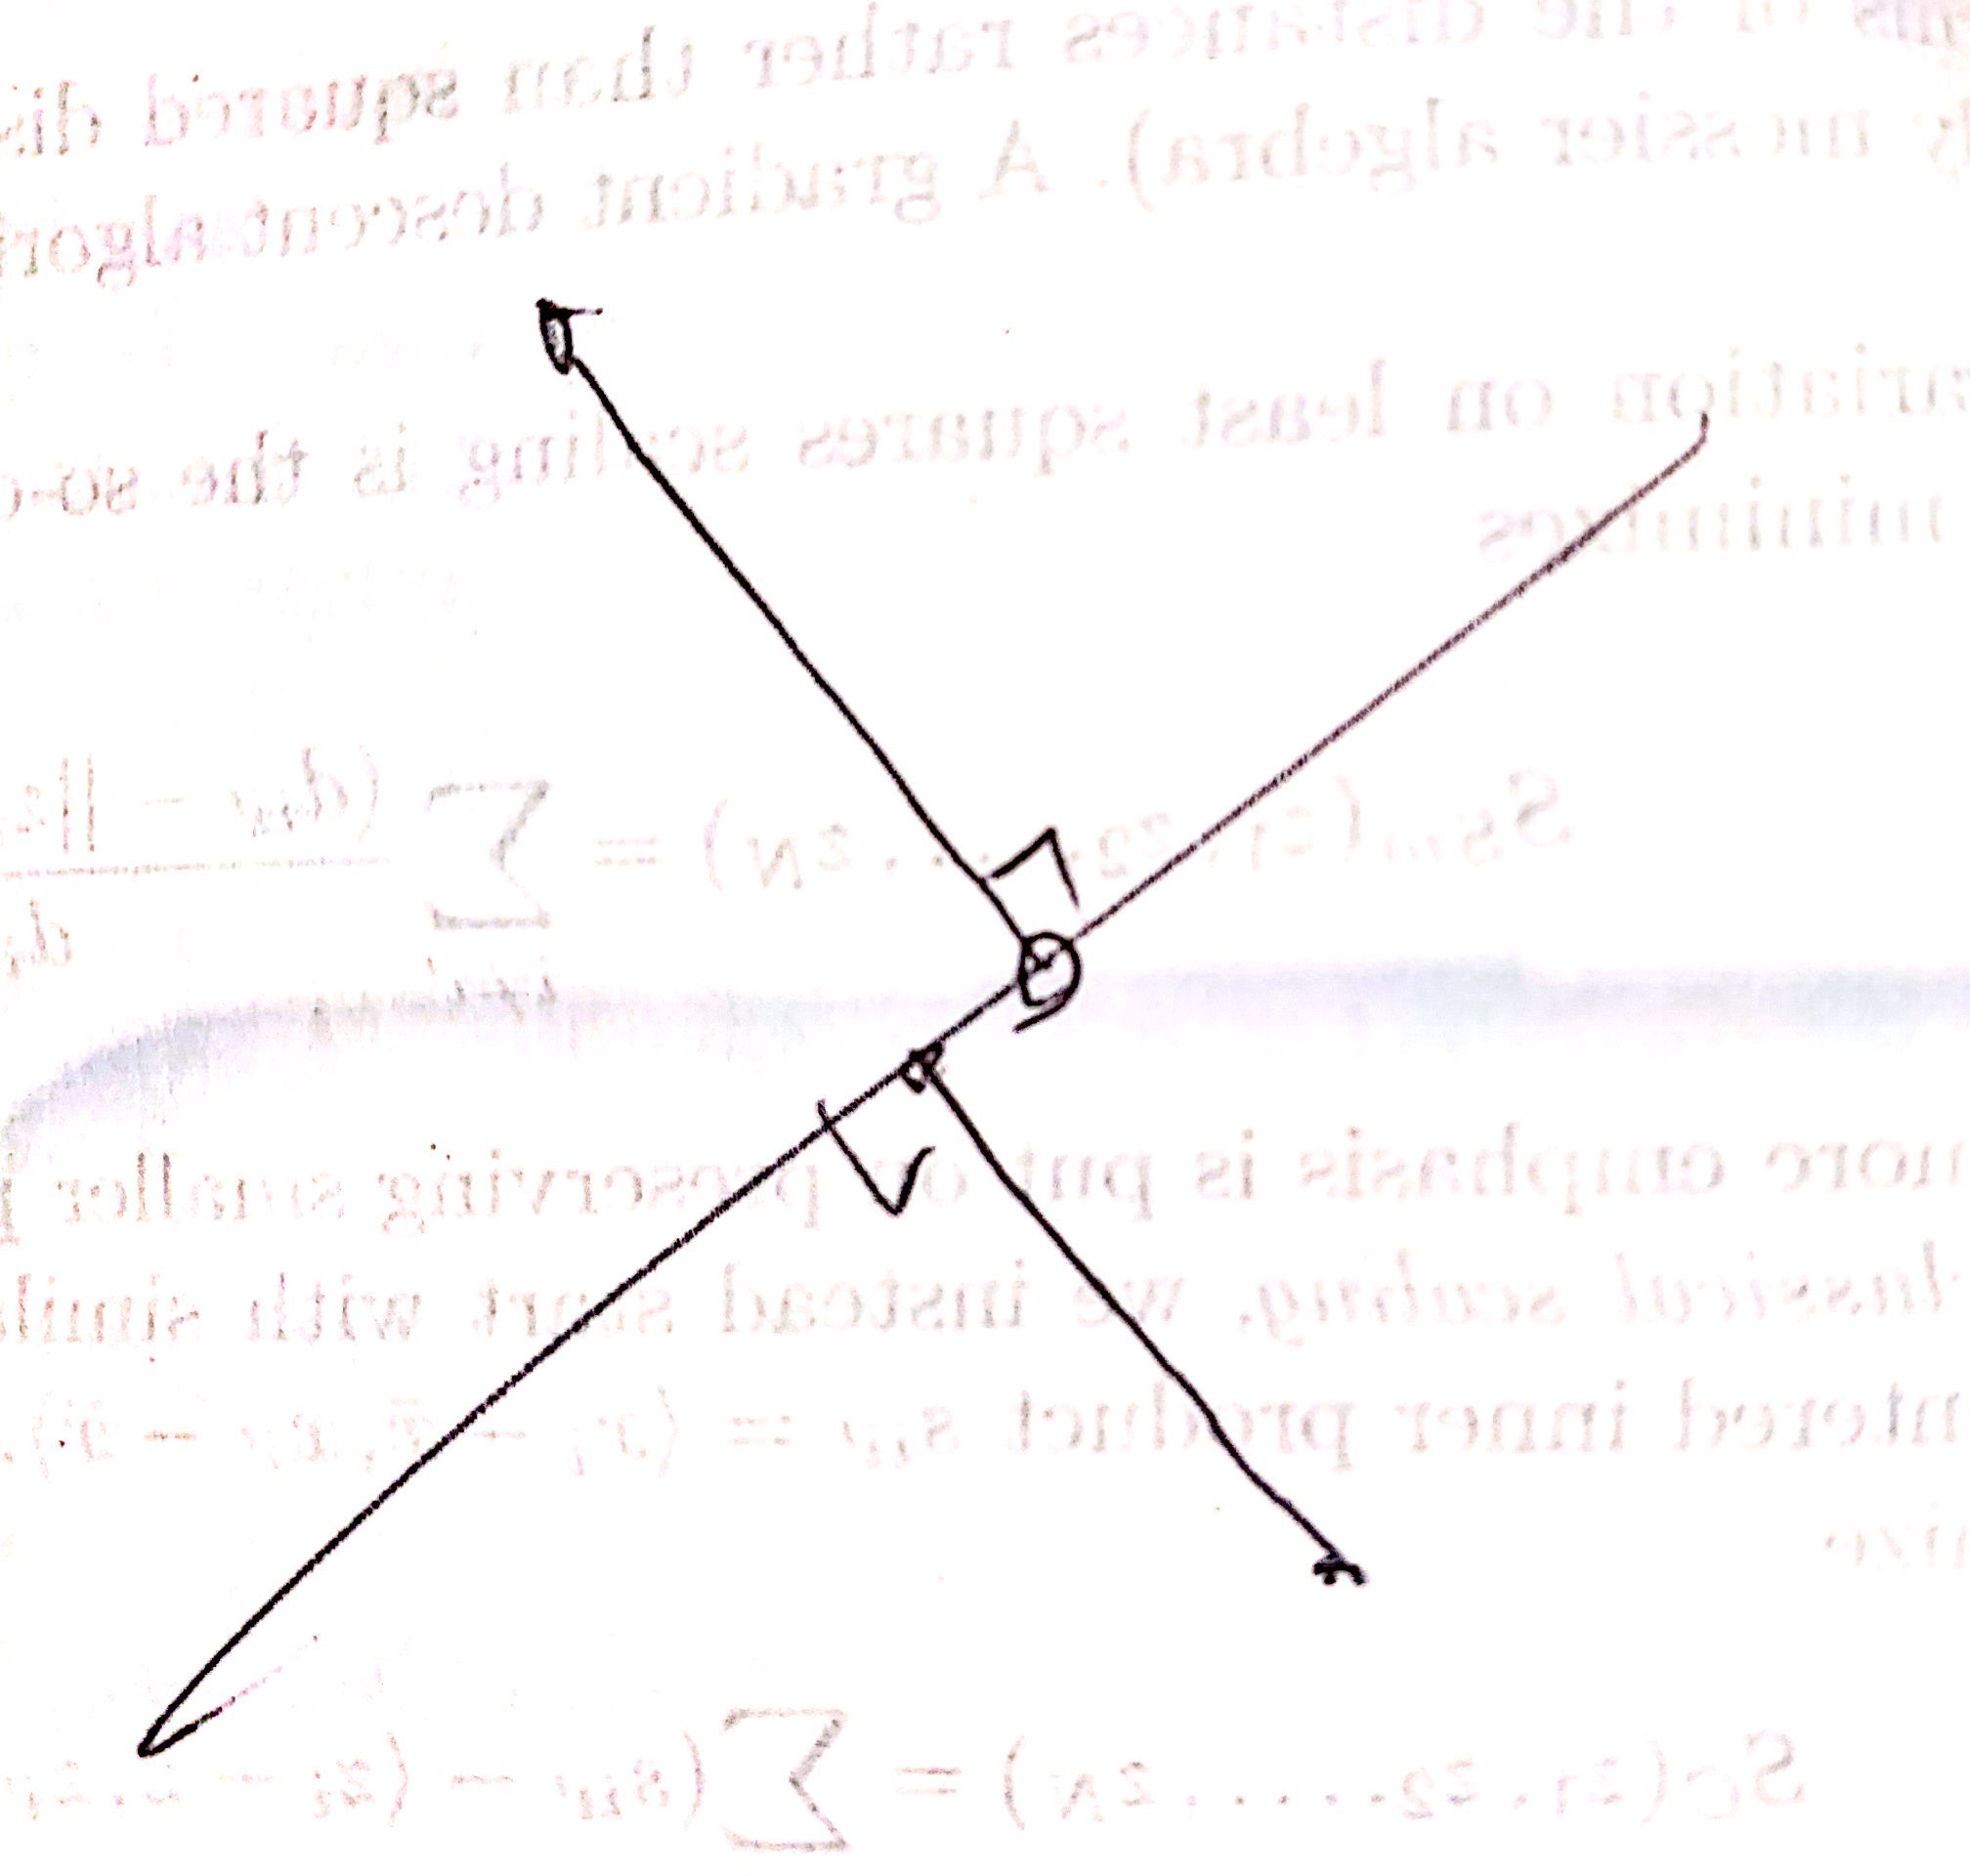
\includegraphics[width=5cm, clip]{images/pca-low-performance.jpg}
        \end{figure}
      \item MDSは, 距離を保存することに主眼を置いているので, 近いものは近く, 遠いものは遠くなる.
    \end{itemize}
  \end{frame}
  \section{非線形次元削減と局所多次元尺度構成法\\p.572-}
  \begin{frame}{非線形次元削減}
    主面のような, 非線形の次元圧縮の方法について.

    多様体面に沿う距離(=測地線の長さ)を測らないと, うまく次元を落とせない. 左の図はうまくいってない例.
    \begin{figure}[htb]
      \centering
      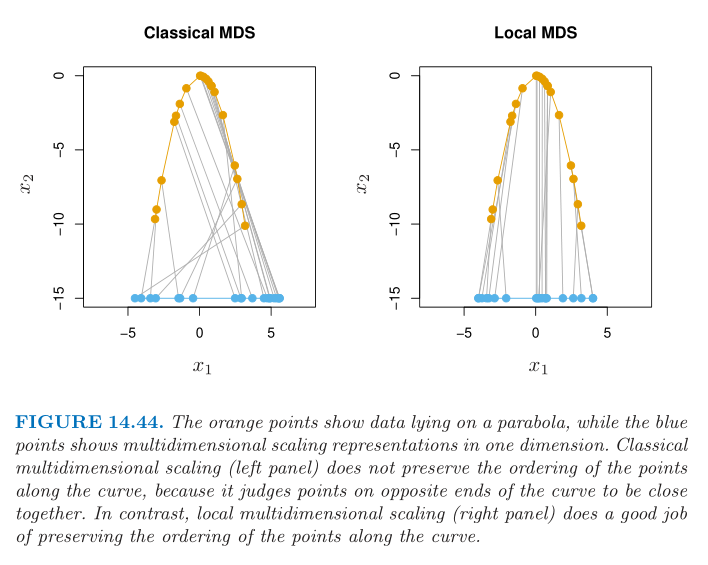
\includegraphics[width=5cm,clip]{images/reducedimension-fail.png}
    \end{figure}

    うまくいかせるためのいくつかの手法を紹介.
    \begin{itemize}
      \item Isometric feature mapping(ISOMAP)
      \item Lacal linear embedding
      \item Local MDS
    \end{itemize}
  \end{frame}
  \begin{frame}{ISOMAP}
    二点間の距離を直接測らず, 点つなぎの要領で足し合わせる. \\
    →疑似的な測地線の長さを得る. \\
    →その距離=非類似度をもとに, Clasical scalingで低次元の空間に点を埋め込む.
  \end{frame}
  \begin{frame}{Local linear embedding}
    各点を近傍の点の線形結合で表す. \\
    →低次元の空間で, その線型結合の関係を可能な限り再現する.

    \begin{enumerate}
      \item 各点$x_i$の$K$近傍$\mathcal{N}(i)$を取る.
      \item 各点を$K$近傍内の点の線形結合として, 可能な限り正確に表現する.
        \[
          \mathrm{minimize} \quad |x_i-\sum_{k\in\mathcal{N}(i)}w_{ik}x_k|^2
        \]
      \item $d < p$次元の空間に点$y_i$を2の線形関係を可能な限り保つようにとる.
        \[
          \mathrm{minimize} \quad \sum_{i=1}^N|y_i-\sum_{k=1}^Nw_{ik}y_k|^2
        \]
    \end{enumerate}
  \end{frame}
  \begin{frame}{Local MDS}
    近傍のペアの集合$\mathcal{N}\subset \{1,\dots,N\}^2$を,
    \[
      (i,i')\in\mathcal{N}\Leftrightarrow x_i\in \mathcal{N}(i')\mbox{かつ}x_i'\in \mathcal{N}(i)
    \]
    とする. ストレス関数を,
    \[
      S_L(z_1,\dots,z_N)=\sum_{(i,i')\in\mathcal{N}}(d_{ii'}-|z_i-z_{i'}|)^2+\sum_{(i,i')\notin\mathcal{N}}w(D-|z_i-z_{i'}|)^2
    \]
    とする. ただし, $D$は大きな定数. つまり, 近傍外の点は非常に遠いものと扱う.
    ただし, 小さな重み$w$を付けて, 影響は小さく.
  \end{frame}
  \section{The Google PageRank Algorithm\\p.576-}
  \begin{frame}{The Google PageRank Algorithm}
    Googleの検索エンジンのアルゴリズムについて.

    $N$個のウェブページを, 重要度順に並べたいとする.
    この``重要度''が``PageRank''と呼ばれるもの.

    基本方針としては, 他のページからのリンクが張られているほど重要と思う.
    ただし, リンクの重みも以下の条件によって変わる.
    \begin{itemize}
      \item リンク元のページの重要度
      \item リンク元のページ内に張られているリンク数
    \end{itemize}

    この考え方を定式化していく.

  \end{frame}
  \begin{frame}{The Google PageRank Algorithm}
    隣接行列$L$.
    \[
      L_{ij}=1 \Leftrightarrow \mbox{ページ}j\mbox{からページ}i\mbox{へのリンクがある}
    \]
    被リンク数$c_j$.
    \[
      c_j=\sum_iL_{ij}=\mbox{他ページへのリンク数}
    \]
    PageRank $p_i$.
    \[
      p_i=(1-d)+d\sum_j\frac{L_{ij}}{c_j}p_j
    \]
    再帰的な定義なので, 実際の計算は反復計算をする.
  \end{frame}
  \section{最後に - 出てきた特徴的な言葉まとめ}
  \begin{frame}{最後に - 出てきた特徴的な言葉まとめ}
    \begin{itemize}
      \item Manifold\\
        多様体. 数学的な概念. 曲線, 曲面, 球面などの進化版.
      \item Dimention reduction\\
        次元削減. 教師なし学習の目的の一つ. 変数の数を減らすこと.
      \item Alternating fashion\\
        最適化アルゴリズムの特徴づけの一つ. パラメータを更新していって最適解に収束させる手法.
      \item Self consistent\\
        自己無撞着, 自己整合. あるものの定義にそのものが含まれるが筋は通っているもののこと.
      \item Subject matter consideration\\
        分析の中で, データからではなく, 背景知識等による考察による部分.
    \end{itemize}
  \end{frame}
\end{document}
